\documentclass[12pt,ngerman,toc=listofnumbered,toc=bibliographynumbered,toc=index,headsepline=true]{scrbook}
\setcounter{secnumdepth}{3}
\setcounter{tocdepth}{3}
\usepackage[T1]{fontenc}
\usepackage[utf8]{inputenc}            % UTF8-Encoding
\usepackage[english, ngerman]{babel}   % deutscher Artikel
% Font mit Umlauten
\usepackage{graphicx}
\usepackage{pdfpages}                  % PDF-Grafiken einbinden
\usepackage{subfig}                    % Subabbildungen
\usepackage{listings}                  % Quellcodes
\usepackage{url}                       % URLs mit Zeilenumbruch
\usepackage{amsmath}                   % Mathematische Symbole

\usepackage[babel,german=quotes]{csquotes}

\usepackage{tikz} 
\usepackage{avant}
\renewcommand{\familydefault}{\sfdefault}

\makeatletter

% \hypersetup{colorlinks=true,linkcolor=black,citecolor=black,filecolor=black,urlcolor=black}
\usepackage[ngerman]{babel}
\usepackage{bibgerm}

\makeatother

\begin{document}
	\frame{\begin{tikzpicture}[remember picture, overlay]%
		\node[anchor=center] at (current page.center){
\includegraphics[width=\paperwidth,height=\paperheight]{versuch1e.png}};
		\end{tikzpicture}} 
	
	
	
	
	
	
	
	
	
	
\thispagestyle{empty}
\selectlanguage{ngerman}
\pagenumbering{Roman}
\newpage
\textcolor{white}{.}
\KOMAoption{headsepline}{false}
\newpage
\textcolor{white}{.}
\newpage
\vspace*{\fill} 
\noindent\hspace*{42mm}%
2015 Oliver Skawronek, Alexander Kern

\noindent\hspace*{42mm}%
http://cactibook.alexkern.de

\noindent\hspace*{42mm}%
E-Mail: cactibook@web.de

\noindent\hspace*{42mm}%
ISBN: 978-3-00-047034-9 

\textcolor{white}{.}
\textcolor{white}{.}
\textcolor{white}{.}

\tableofcontents
\KOMAoption{headsepline}{true}
\newpage
\pagenumbering{arabic}

\setlength{\parindent}{0pt} % Absatzeinzug
\setlength{\parskip}{1.0ex} % Absatzabstand

%Code Style
\lstset{ %
%language=Java,                % choose the language of the code
basicstyle=\footnotesize,      % the size of the fonts that are used for the code
tabsize=2,	                   % sets default tabsize to 2 spaces
breaklines=true,               % sets automatic line breaking
breakatwhitespace=false,       % sets if automatic breaks should only happen at whitespace
showstringspaces=false
}



\chapter{Einleitung}
Der Betrieb eines Netzwerkes erfordert u.\,a. die Überwachung von
Netzwerkkomponenten. Cacti ist eine open-source Softwarelösung für diese
Aufgabe. In Cacti werden in regelmäßigen Abständen Werte von Netzwerkkomponenten
aufgezeichnet und dem Benutzer als Graphen präsentiert. Cacti kann u.\,a.
Kapazitätsengpässe grafisch hervorheben und erlaubt damit ein schnelles
Reagieren in kritischen Situationen.

Unter einer Weboberfläche kombiniert Cacti verschiedene Technologien zum
Erfassen, Speichern und Darstellen von Messwerten. Vorhandene Detailkenntnisse
in den Technologien sind nicht Voraussetzung zur Nutzung. Cacti bietet hierzu
Voreinstellungen für Standardaufgaben,  bspw. für das Überwachen der Netzlatenz
mittels Ping. Erfahrene Benutzer können jedoch individuelle Einstellungen
treffen.

Ziel dieser Arbeit ist es dem Leser einen Überblick über Cacti zu geben, die
Funktionalität zu erläutern und anhand eines privaten Homeservers
Einsatzmöglichkeiten aufzuzeigen.\\
In der Arbeit werden die Prinzipien der Messdatenerfassung sowohl mittels Script
als auch mittels SNMP beschrieben und sind mit Beispielen unterlegt. Weiterhin
wird erläutert, wie Cacti die Messdaten mit konstantem Speicherplatz
persistiert, und welche Komponenten für die Messdatendarstellung angeboten
werden.\\
Kapitel \ref{sec:Anwendungsbeispiel} zeigt, dass gängige
Server-Software, wie der Apache2-Webserver, Metriken typischerweise in Form von
Log-Dateien bereitstellen. Durch Kommandozeilenprogramme, wie grep und awk, lassen sich die
Metriken in das von Cacti gewünschte Format überführen, und letztlich in Form von Graphen
visualisieren. Für das Bereitstellen von Messdaten per SNMP zeigt Kapitel
\ref{sec:MIB} die Implementierung eines MIB-Moduls für Net-SNMP.

\chapter{Überblick}
Cacti ist eine Webanwendung zum Erfassen, Speichern und Darstellen von
Messwerten. Hauptsächlich wird Cacti im Bereich des Netzwerkmonitorings
eingesetzt. Über eine Weboberfläche erfolgt die Administration. Hier können die
zu überwachenden lokalen oder entfernten Netzwerk-Geräte, wie Server, Router und
Switches, verwaltet werden. In regelmäßigen Abständen ruft Cacti die Messdaten
dieser Geräte ab und speichert sie langfristig in Archiven. Neben der Abfrage
über Scripts können die Daten auch aus Anfragen über das \textit{Simple Network
Management Protocol} (SNMP) stammen. Aus ausgewählten Messdaten
(gesendete/empfangene Bytes, erfolgreiche/fehlgeschlagene Anmeldungen etc.)
werden Graphen erstellt und auf der Weboberfläche präsentiert.

Für den Einsatz in größeren Netzumgebungen, bspw. in Rechenzentren, erleichtert
Cacti die Verwaltung gleichartiger Netzkomponenten durch sogenannte
\enquote{Templates}. Die Idee dabei ist, für eine Geräteklasse (ggf. eines
bestimmten Herstellers) in einem Template festzulegen, welche Messdaten erfasst
und dargestellt werden sollen. Wird ein neues Gerät dieser Klasse in die
Netzumgebung installiert, werden zu diesem Gerät alle benötigten Graphen
automatisch erstellt.

Cacti unterstützt den Mehrbenutzerbetrieb. Durch Vergabe von Nutzerrechten lässt
sich festlegen, welche Einstellungen ein Benutzer treffen kann und welche
Graphen ihm angezeigt werden. Die Anmeldung erfolgt über die Weboberfläche und
kann sowohl lokal als auch entfernt über einen Browser geschehen.

\section{Einsatzmöglichkeiten}
Cacti bietet eine Vielzahl von Einsatzmöglichkeiten, von denen im Folgendem
einige herausgegriffen werden:

\textbf{Technische Einsatzmöglichkeiten}
\begin{itemize}
  \item Auslesen von Log-Dateien. Im Kapitel \ref{sec:Anwendungsbeispiel} werden
  dazu Beispiele vorgestellt.
  \item Benachrichtigung via E-Mail, wenn kritische Werte über- bzw.
  unterschritten werden. Hierfür ist ein zusätzliches Plug-In einzubinden.
  \item Einige Datenbank-Managementsysteme bieten die Abfrage von Metriken, wie
  Verbindungen, Sperren und Cache-Misses, via SNMP an. Diese Metriken lassen
  sich schließlich mit Cacti überwachen.
\end{itemize}

\textbf{Einsatzmöglichkeiten im Netzwerk- und Systemmanagement}
\begin{itemize}
  \item Überwachen der Einbruchsversuche durch Anbindung an ein Firewallsystem
  \item Darstellung des Netzwerkverkehrs sowie der Speicher- und Prozessorauslastung
  \item Überwachen der Signalstärke von WLAN-Stationen
  \item Abfrage der Metriken von Proxyservern, Routern, VoIP-Telefonanalagen
  etc.
  \item Statistische Auswertung des E-Mailverkehrs (Speicherverbrauch, Spam,
  usw.)
  \item Über"-wa"-chen der Aus"-las"-tung ein"-zel"-ner Pro"-zes"-sor"-ker"-ne. Auf Grund"-lage die"-ser Messungen können Kaufentscheidungen getroffen werden, bspw. ob sich die Anschaffung weiterer Mehrkernprozessoren unter der einge"-setz"-ten Software lohnt.
  \item Gegenüberstellung des Verbrauchs unterschiedlicher Ressourcenkategorien, wie Anwendungsdaten und Media.
\end{itemize}

\section{Messdatenerfassung}
Die Messdatenerfassung erfolgt regelmäßig in festen Abständen (standardmäßig im
Fünf-Minuten-Takt) über den sogenannten \enquote{Poller}. Dazu werden Scripts
und Anfragen über SNMP ausgeführt und die ermittelten Messwerte gespeichert. Unter
Linux wird bspw. der Poller als Cronjob\footnote{Ein Cronjob ist unter Linux
eine sich wiederholende Aufgabe. Er besteht aus der Angabe des aufzurufenden
Befehls und dem zeitlichen Abstand zwischen zwei Aufrufen.} aufgerufen. Cacti
bietet zum Erfassen von Messdaten mehrere Möglichkeiten an:
\begin{itemize}
  \item Data-Input-Methods: Abfrage skalarer Werte, bspw. der
  Umgebungstemperatur eines Switches. Die Werte können von der Ausgabe eines
  Scripts oder einer SNMP-Abfrage stammen.
  \item Data-Querys: Abfrage Index-basierter Werte. Die Daten stammen aus einer
  Tabelle. Jeder Tabellenzeile ist ein eindeutiger Indexwert zugewiesen.
  Beispielsweise könnte ein Host in einer Tabelle die gesendeten und empfangenen
  Daten aller installierten Netzwerkadapter anbieten, wobei jedem Netzadapter
  ein Laufindex zugeordnet ist. Abgefragt werden die Daten entweder per Script
  oder SNMP.
\end{itemize}

\section{Messdatenspeicherung}
Die langfristige Speicherung von Messdaten ist mit einem ständig wachsenden
Speicherplatzbedarf verbunden. Misst man bspw. aller fünf Minuten die Ping-Zeit,
so müssen $12$ Messpunkte pro Stunde, $12*24 = 288$ Messpunkte pro Tag, $288*365=
105120$ Messpunkte pro Jahr usw. gespeichert werden. Während man aktuelle
Messdaten über kurze Zeitabstände betrachten möchte, genügt typischerweise nur
ein Überblick über ältere Werte. Beispiel:
\begin{itemize}
  \item Aller fünf Minuten wird ein Messwert erfasst.
  \item 12 Messwerte werden zu einem konsolidierten
  \enquote{Stunden-Messwert},
  \item 24 \enquote{Stunden-Messwerte} zu einem konsolidierten
  \enquote{Tages-Messwert}, usw. zusammengefasst.
%  \item 7 \enquote{Tages-Messwerte} zu einem konsolidierten
%  \enquote{Wochen-Messwert},
%  \item 4 \enquote{Wochen-Messwert} zu einem konsolidierten
%  \enquote{Monats-Messwert} usw. zusammengefasst.
\end{itemize}

Aktuelle Werte werden somit in einer höheren Auflösung als ältere Werte
gespeichert. Mögliche Konsolidierungsfunktionen sind:
\textit{Mittelwert}, \textit{Maximum}, \textit{Minimum} usw.

In Cacti werden die erfassten Messwerte nach diesem Prinzip abgespeichert. Dazu
basiert Cacti auf dem RRDTool (RRD für Round Robin Database). Es garantiert für
die gewählte Zeitauflösung einen konstanten Platzbedarf zur Speicherung der
Messwerte.

Data-Input-Methods bzw. Data-Querys dienen der Abfrage von Messwerten. Die
sogenannten \enquote{Data-Sources} legen hingegen fest, wie die Messdaten in den
Round-Robin-Datenbanken (RRDs) gespeichert werden. Diese RRDs speichern mehrere
Messgrößen in Archiven unterschiedlicher Auflösung ab. Eine zu speichernde
Messgröße, bspw. die empfangenen Byte eines Netzwerkadapters, entspricht in
Cacti einem \enquote{Data-Source-Item}. Mehrere Data-Source-Items sind einer
Data-Source zugeordnet. Die Data-Source legt hauptsächlich fest, welche Archive
(Stunden-Archiv, Tages-Archiv, Wochen-Archiv usw.) für die Messgrößen angelegt
werden und bestimmt damit das Schema der zugeordneten RRD.

\section{Messdatendarstellung}
Das RRDTool dient Cacti neben der Speicherung der Messwerte auch zum Erstellen
der Messdatendarstellung in Form von Graphen. Mehrere Messgrößen lassen sich in
einem Graph darstellen. Neben der Möglichkeit, Titel, Legende,
Achsenbeschriftung, Farbe etc. festzulegen, ist hier die Fähigkeit von RRDTool
hervorzuheben, mathematische Funktionen auf die Eingabegrößen anzuwenden. Damit
können bspw. einfache Größenumrechnungen, wie von Bit/s nach Byte/s, umgesetzt
werden. Die Bestandteile eines Graphen, wie eine darzustellende Messgröße oder
die Einträge in der Legende, werden als \enquote{Graph-Items} bezeichnet.

\section{Templates}
Insbesondere der angebotene Template-Mechanismus erleichtert den Einstieg
Netzressourcen mit Cacti zu überwachen, da Detailkenntnisse über Data-Sour"-ces
u.\,Ä. nicht vorausgesetzt werden.

Es werden drei Arten von Templates unterschieden:
\begin{enumerate}
  \item Data-Templates: Sie kommen zum Einsatz, wenn mehrere Data-Sources
  gleiche Charakteristika teilen. Auf diese Weise werden automatisch mit jeder
  Data-Source (die auf einem Data-Template basiert) die zugehörigen
  Data-Source-Items angelegt.
  \item  Graph-Templates: Mittels Graph-Templates lassen sich einheitlich
  aussehende Graphen erstellen. Titel, Legende, Achsenbeschriftung etc. werden
  in einem Graph-Template einmal festgelegt, und alle daraus abgeleiteten
  Graphen erben diese Eigenschaften.
  \item Host-Templates: Einem Host-Template sind eine Menge von Data-Temp"-lates
  und Graph-Templates zugeordnet. Angelegt werden Host-Templates für
  gleichartige Geräteklassen. Wird ein Gerät einer solchen Geräteklasse der
  Netzumgebung hinzugefügt, können automatisch alle Data-Sources zur
  Messdatenerfassung und Graphs zur Messdatendarstellung erstellt werden.
\end{enumerate}
% http://docs.cacti.net/templates
Durch den Template-Import und -Export ist es möglich, Templates zu verteilen.
Beispielsweise werden unter \cite{Cacti11} Templates für \enquote{Cisco-Router}
zum Download angeboten.

\section{Benutzerverwaltung}
Mit jeder Standardinstallation von Cacti werden die Nutzer \enquote{admin} und
\\ \enquote{guest} angelegt. Weitere Benutzer lassen sich hinzufügen. Jedem
Benutzer ist ein Benutzername und Kennwort zugeordnet sowie eine Menge von
Benutzerrechten. Die Benutzerrechte legen fest, welche Einstellungen in Cacti
von einem Benutzer getroffen werden können und welche Graphen für ihn sichtbar
sind.

\section{Plug-Ins}
Es existiert eine Vielzahl an Plug-Ins für Cacti. Über sie können zusätzliche
Informationen angezeigt, Funktionen ergänzt und Daten und Graphen manipuliert
werden. Beispielsweise dient das Plug-In \enquote{Thold} \cite{Conner11} der
Überwachung von Messgrößen. Überschreitet ein Messwert einen bestimmten
Schwellwert, etwa eine zu hohe Festplattenauslastung, kann Thold automatisch den
Administrator per E-Mail darüber benachrichtigen.

Cacti kommuniziert über sogenannte \enquote{Hooks} mit den Plug-Ins. Hooks sind
Call-Back-Funktionen, für die sich jedes Plug-In registrieren muss. Cacti ruft
diese Funktionen auf und übergibt Informationen in Form von Argumenten. Soll ein
Plug-In bspw. auf Statusänderungen eines Geräts reagieren, muss es sich für den
Hook \enquote{Update-Host-Status} registrieren und eine gleichnamige Funktion
implementieren.

\section{System-Architektur}
% Urban11, Seite 2 (System architecture of Cacti)
Zur Abfrage nutzt Cacti einen Cronjob-basierten Poller um Daten aus
verschie"-denen Quellen abzufragen. Die abgefragten Daten werden in RRD-Da\-teien
gespeichert. Alle Einstellungen zur Systemkonfiguration werden in
My\-SQL-Tabel"-len gehalten. Sowohl die Konfiguration als auch die Darstellung der
Graphen auf der Weboberfläche wurde hauptsächlich in der Scriptsprache PHP
implementiert. Cacti ist u.\,a. für Windows, Linux und Solaris verfügbar
\cite{Urban11}.

\chapter{Messdatenerfassung}
Zu den grundsätzlichen Aufgaben in Cacti zählen die Messdatenerfassung,
-Speicherung und –Darstellung. In diesem Kapitel werden die unterschiedlichen
Möglichkeiten der Messdatenerfassung mit Cacti vorgestellt. Die Messdaten können
von verschiedenen, ggf. entfernten Quellen stammen. Im Bereich des
Netzwerkmonitorings ist vor allem die Möglichkeit zu nennen,  Messwerte
mittels SNMP abzufragen. Eine Vielzahl an Netzwerk-Geräten, wie Switches, 
Router und Drucker, unterstützten dieses Protokoll. Neben SNMP bietet Cacti an,
Daten über Scripte abzufragen. Das bedeutet, der Ausgabestrom von Linux-Befehlen
bzw. Linux-Scripts kann ausgelesen werden. Daneben besteht die Möglichkeit,
direkt PHP-Scripts auszuführen.

Die Messdatenerfassung ist konzeptmäßig von der -Speicherung und
-Dar\-stel\-lung getrennt. Für die weitere Verarbeitung werden die Messwerte in
ein einheitliches Format kodiert, d. h. es muss nicht beachtet werden, aus
welcher Quelle die Daten stammen. Die einzige Vorrausetzung ist, dass die Werte
ganzzahligen oder reellwertigen Datentypen zugeordnet sind.

Abgerufen werden die Messwerte in einem festen Intervall durch den Poller. Wie
der Name bereits erahnen lässt, wird die aktive Abfragemethode \enquote{Polling}
umgesetzt, d.\,h. die Geräte senden auf Anfrage ihre Werte an Cacti. Standardmäßig
führt der Poller im Fünf-Minuten-Takt die SNMP-Anfragen bzw.
Scripts aus, und speichert anschließend die Werte in Archiven ab. Sind die
Messgrößen einem bestimmten Gerät zugeordnet, prüft der Poller zusätzlich, ob
das Gerät noch aktiv ist, bspw. durch eine Ping-Anfrage.\\
Es existieren zwei Implementierungen des Pollers:
\begin{enumerate}
  \item cmd.php: In PHP implementierter Standard-Poller.
  \item Spine: In C implementierter Poller.
\end{enumerate}
%Urban11, S. 16, Installing the Spine poller
\textsc{Urban} empfiehlt in \cite{Urban11} cmd.php für kleine bis mittelgroße
Netzumgebungen. Für große Netzumgebung sollte hingegen Spine eingesetzt werden.
Das ist u.\,a. damit zu begründen, dass Spine multitaskingfähig ist.

Je nach Art der abzufragenden Daten wird zwischen Data-Input-Methods und
Data-Querys unterschieden:
\begin{itemize}
  \item Data-Input-Methods: Abfrage eines oder mehrere skalarer, nicht
  indexbasierter Werte.\\
  Beispiele: Temperatur, Speicherverbrauch, Anzahl eingeloggter Benutzer, Anzahl
  empfangener/gesendeter Pakete, Anzahl erfolgreicher/ abgebrochener
  Datenbank-Transaktionen
  \item Data-Querys: Abfrage indexbasierter Werte. Die Werte werden aus einer
  Tabelle ausgelesen, wobei jeder Tabellenzeile ein eindeutiger Indexwert
  zugewiesen ist.\\
  Beispiele: Liste mit Netzwerkkarten (Verbindungsgeschwindigkeit,
  empfangene/gesendete Pakete usw.), Liste mit Festplatten (Gesamtkapazität,
  Verfügbarer Speicher usw.)
\end{itemize}
Für beide Arten werden im Folgenden Möglichkeiten aufgezeigt, Werte über Scripts
oder SNMP abzufragen.

\section{Abfrage Script-basierter Messwerte}
\label{subsec:AbfrageScript}
Das Auslesen Script-basierter Daten erlaubt in Verbindung mit den
Kom\-man\-dozeilen-Befehlen \enquote{awk}, \enquote{grep}, \enquote{wc} u.\,a. 
eine Reihe einfacher Abfragen auf Textdateien, wie Server-Logs. Kombiniert werden
diese Befehle häufig über Pipes, d.\,h. der Ausgabestrom des vorhergehenden
Befehls dient als Eingabe für den nächsten Befehl. In diesem Abschnitt soll
anhand von Beispielen erklärt werden, in welchem Format letztlich die Ausgabe
vorliegen muss, damit Cacti sie einlesen kann, und wie die Scripts gesteuert werden.

\textbf{Beispiel}\quad Einlesen eines einzelnen Wertes:\\[1ex]
Der Einfachheitshalber soll mittels Echo-Befehl der konstante Wert $10,45$
ausgegeben werden:
\begin{lstlisting}[xleftmargin=20pt]
echo '10.45'
\end{lstlisting}
Zum Einlesen des Wertes muss eine neue Data-Input-Method mit dem
Input-Type \enquote{Script/Command} erstellt werden (siehe Abbildung
\ref{fig:echoinputmethod}). Im Feld Input-String ist der auszuführende Befehl
bzw. der Pfad zum auszuführenden Script anzugeben.

\begin{figure}
	\centering
	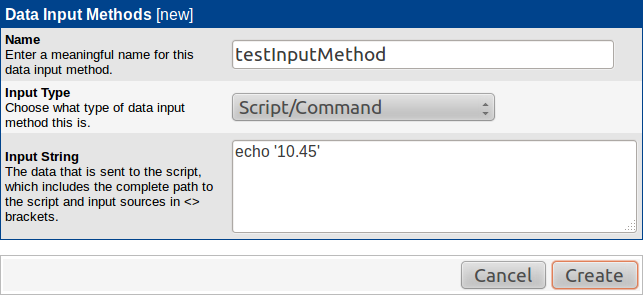
\includegraphics[scale=0.5]{bilder/echoinputmethod}
	\caption{Auslesen eines Wertes mittels Data-Input-Method}
	\label{fig:echoinputmethod}
\end{figure}

Einer Data-Input-Method sind eine Menge von Input- und Output-Fields zugeordnet.
Dabei sind Input-Fields im Falle von Scripts als Übergabeparameter
aufzufassen. Output-Fields sind die auszulesenden Messgrößen, d.\,h. die Werte,
die Cacti mit jedem Polleraufruf aus dem Ausgabestrom des Scripts ermittelt. Es
muss mindestens ein Wert ermittelt werden. In Folge muss auch mindestens ein
Output-Field einer Data-Input-Method zugeordnet sein. Die Anzahl an zugeordneten
Input-Fields ist jedoch beliebig.

Das Script aus dem obigen Beispiel hat keine Eingabeparameter und einen
Ausgabewert, d.\,h. es muss ein Output-Field angelegt werden, wie in Abbildung
\ref{fig:echooutputfield} gezeigt. Nach diesem Schritt ist Cacti in der Lage,
den einzelnen Wert mit jedem Polleraufruf abzufragen und ihn anschließend in
einem Archiv zu speichern sowie in einem Graph darzustellen.

\begin{figure}
	\centering
	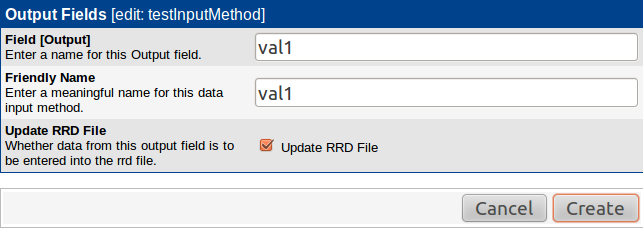
\includegraphics[scale=0.5]{bilder/echooutputfield}
	\caption{Der Data-Input-Method wird ein Output-Field hinzugefügt}
	\label{fig:echooutputfield}
\end{figure}

\textbf{Beispiel}\quad Auslesen von Ping-Statistiken:\\[1ex]
Zur Demonstration, wie mehrere Input- und Output-Fields genutzt werden können,
sollen mit einer Data-Input-Method Ping-Statistiken ausgelesen werden. Einem
Host werden mehrere Echo-Request-Pakete gesendet. In den Statistiken wird
ausgewertet, wie viele davon nicht durch Echo-Reply-Pakete von ihm beantwortet
wurden (Paketverlust) und welche Zeit insgesamt dazu benötigt
wurde.

Eine Anfrage sieht wie folgt aus:

\begin{lstlisting}[xleftmargin=20pt]
ping -c 5 google.de
\end{lstlisting}

Hier werden dem Host \textit{google.de} fünf Echo-Request-Pakete gesendet. Der
Ping-Befehl gibt daraufhin folgendes aus:

\begin{lstlisting}[xleftmargin=20pt]
...
--- google.de ping statistics ---
5 packets transmitted, 5 received, 0% packet loss, time 4013ms
rtt min/avg/max/mdev = 14.578/20.870/25.298/4.008 ms
\end{lstlisting}

Für das Beispiel ist die Zeile interessant, in der der Paketverlust und die
benötigte Zeit steht.

Im vorherigen Beispiel wurde nur ein Wert ausgelesen. Sollen mehrere
Werte ausgelesen werden, d.\,h. der Data-Input-Method sind auch mehrere
Output-Fields zugeordnet, erwartet Cacti den einzulesenden Ausgabestrom in
folgendem Format:
\begin{lstlisting}[xleftmargin=20pt]
<fld_1>:<val_1> <fld_2>:<val_2> ... <fld_n>:<val_n>
\end{lstlisting}
Also eine Leerzeichen-separierte Liste von Feldname-Wert-Paaren.\\
Für das Umformatieren obiger Ausgabe bietet sich das Programm \enquote{awk} an.
Es kann Textstellen mit regulären Ausdrücken aufsuchen und in ein anderes Format
ausgeben:

\begin{lstlisting}[xleftmargin=20pt]
ping -c <packageCount> <host> |
awk '/transmitted/ {match($0,
  /([[:digit:]]+)% packet loss, time ([[:digit:]]+)ms/,
  groups);
printf("loss:%d time:%d", groups[1], groups[2])}'
\end{lstlisting}

Mittels Pipe \enquote{\texttt{|}} wird die Ausgabe von ping an awk
weitergeleitet. Daraufhin sucht awk alle Zeilen, die das Wort
\enquote{transmitted} enthalten. Bei jeder gefundenen Zeile werden die in
geschweiften Klammern \enquote{\texttt{\{\ldots\}}} angegebenen Aktionen
ausgeführt. Mittels \enquote{match}-Befehl werden die interessanten Werte in das
Array \enquote{groups} geschrieben, und mittels \enquote{printf}-Befehl neu
formatiert. Letztlich sieht die umformatierte Ausgabe wie folgt aus:

\begin{lstlisting}[xleftmargin=20pt]
loss:0 time:4013
\end{lstlisting}

Damit die Abfrage flexibel bleibt, 
wurden die Übergabeparameter in 
spit"-zen
Klammern \enquote{\texttt{<\ldots>}} angegeben: \texttt{-c <packageCount>
<host>}. Diese müssen durch Input-Fields modelliert werden. Beim Anlegen einer
Data-Source für das Speichern der Werte müssen den Input-Fields schließlich konkrete
Argumente zugeordnet werden. Zudem ist es möglich, einen regulären Ausdruck den
Input-Fields zuzuordnen. Damit prüft Cacti, ob die Argumente einem bestimmten
Format entsprechen. Im Beispiel ist der reguläre Ausdruck \texttt{[0-9]+} für
\enquote{packageCount} sinnvoll, damit nur positive, ganzzahlige Werte übergeben
werden dürfen.

Zusammengefasst besteht die Data-Input-Method aus:
\begin{itemize}
  \item Input-Field \enquote{packageCount}: Anzahl an Echo-Request-Paketen
  \item Input-Field \enquote{host}: Host, an den die Pakete gesendet werden
  sollen
  \item Output-Field \enquote{loss}: Paketverlust in Prozent
  \item Output-Field \enquote{time}: Benötigte Zeit in Millisekunden
\end{itemize}
Damit ist es möglich, von einem beliebigen Host Ping-Statistiken abzufragen und
in einem Graphen darzustellen.

\section{Abfrage SNMP-basierter Messwerte}
\subsection{SNMP-Grundlagen}
SNMP ist die Abkürzung für \textit{Simple Network Management Protocol}. In den
Aufgabenbereich dieses Protokolls fällt die Verwaltung entfernter,
netzwerkfähiger Geräte. Es können einerseits Statusinformationen abgefragt,
andererseits Konfigurationen getroffen werden. Beispielsweise ist es möglich,
entfernt die Temperatur eines Switches abzufragen oder eine Netzwerkkarte eines
Routers zu deaktivieren. Das Adjektiv \enquote{simple} bezieht sich auf die
Menge an SNMP-Operationen. Das Protokoll liegt aktuell in der
Version 3 vor und wird im Request for Comments (RFC) 3410 \cite{RFC3410}
beschrieben. Entwickelt wurde SNMP von der Internet Engineering Task Force
(IETF), die auch für das Internet Protocol (IP) und Transmission Control
Protocol (TCP) zuständig ist.\\
Aufgrund der weiten Verbreitung von SNMP bei netzwerkfähigen Geräten, wie
Router, Switches, Drucker aber auch Datenbanksystemen sollen in diesem Abschnitt
die Grundlagen zu SNMP gelegt werden. Aufbauend darauf wird im nächsten
Abschnitt der Einsatz in Cacti gezeigt.

\textbf{Kommunikationspartner}\\[1ex]
Grundsätzlich werden in SNMP zwei Kommunikationspartner definiert:
\textit{Managers} und \textit{Agents} (siehe Abbildung \ref{fig:manageragent};
die Befehle, wie \texttt{GetRequest}, werden unter \enquote{SNMP-Operationen}
erläutert).
Ersterer wird auch als \enquote{Network Management Station} (NMS) bezeichnet. Er
ist für das Polling (mittels Get-Anfragen) und das Empfangenen von sogenannten
\enquote{Traps} zuständig. Ein Agent ist ein Programm, das auf dem zu
verwaltenden Netzwerkgerät läuft. Er stellt den NMS Verwaltungsinformationen
über das Gerät zur Verfügung. Beispielsweise überwacht er permanent den Status
einer Netzwerkkarte in einem Router und kann die aktuelle
Übertragungsgeschwindigkeit bereitstellen. Weitere Aufgaben sind das versenden
von Traps und das Treffen von Einstellungen, wobei diese Aufgaben nicht in den
Bereich von Cacti fallen.\\
Traps sind asynchron versendete Benachrichtigungen an die NMS, bspw. dass ein
Switch gerade hoch/herunter gefahren ist. Sie werden eigenständig von den Agents
versendet. Da sie nicht von der NMS bestätigt werden, gibt es jedoch keine
Garantie für den Empfang.

\begin{figure}
	\centering
	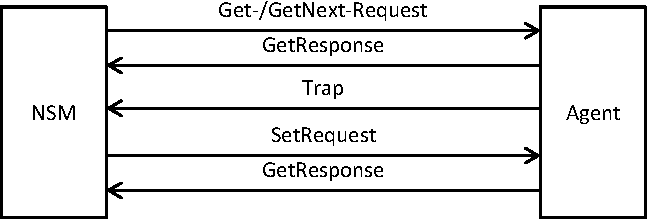
\includegraphics{bilder/manageragent}
	\caption{Network Management Station (NSM) und Agent}
	\label{fig:manageragent}
\end{figure}

\textbf{Managed-Objects}\\[1ex]
% O'Reilly, SNMP, S. 19  
In der Terminologie von SNMP werden die Werte, die abgefragt bzw. gesetzt
werden können, als \enquote{Managed-Objects} bezeichnet. Beispielsweise wird die
aktuelle Anzahl an gestarteten Prozessen als ein Managed-Object bezeichnet. Nach
\cite{Mauro01} lassen sich Managed-Objects durch folgende drei Eigenschaften
beschreiben:
\begin{enumerate}
  \item Name: Der Name, auch \enquote{Object-Identifier} (OID) genannt,
  identifiziert ein Managed-Object eindeutig. Dabei sind zwei Notationen für
  OIDs gebräuchlich: Eine 1) numerische und eine 2) textuelle Notation.
  Beispiel: \texttt{.1.3.6.1.\-2\-.1.\-25.\-1.6.0} (numerisch) und \\  \texttt{iso.org.\-dod.\-in\-ter\-net.mgmt.mib-2.host.hrSystem.hrSystemProcesses}
  (textuell). Beide OIDs identifizieren dasselbe Managed-Object.
  \item Typ und Syntax: Jedem Managed-Object ist ein Datentyp zugeordnet.
  Datentypen werden durch die Beschreibungssprache \enquote{Structure of
  Management Information} (SMI), einer Teilsprache der \enquote{Abstract Syntax
  Notation One} (ASN.1), definiert. Neben den vordefinierten Datentypen, etwa
  \enquote{BOOLEAN}, \enquote{INTEGER} und \enquote{UTF8String}, lassen sich mit
  ASN.1 komplexe Datentypen eindeutig beschreiben.
  \item Enkodierung: Die mit ASN.1 beschriebenen Datentypen sind
  plattformunabhängig. Deshalb ist eine Zuordnung der in ASN.1
  definierten Strukturen (abstrakte Syntax) zu Bit-Mustern für die Übertragung
  (Transfer-Syntax) nötig. Bei SNMP erfolgt die Kodierung der abstrakten Syntax
  zur Transfer-Syntax durch sogenannte \enquote{Encoding Rules}, die in den
  \enquote{Basic Encoding Rules} (BER) definiert sind. Mit BER wird also
  festgelegt, wie Managed-Objects enkodiert/dekodiert werden, damit sie über ein
  Medium verschickt werden können.
\end{enumerate}
OIDs werden in einer Baum-Struktur verwaltet. Es liegt daher nahe, jedem Knoten
nach seiner Position im Baum zu benennen. Von der Wurzel an beginnend, setz
sich die OID eines Knotens aus seinen Namen und den Namen seiner Vorgänger
zusammen, wobei sie jeweils durch einen Punkt \enquote{\texttt{.}} getrennt sind.
Im Beispiel
\texttt{iso.org.\-dod.\-in\-ter\-net.mgmt.mib-2.host.hrSystem.hr\-Sys\-tem\-Pro\-ces\-ses}
ist \texttt{iso} die Wurzel, \texttt{org} der sechste Vorgänger, \texttt{dod}
der fünfte Vorgänger usw. im Baum.

\textbf{SNMP-Operationen}\\[1ex]
SNMPv1 definiert folgende Operationen:
\begin{itemize}
  \item \texttt{GetRequest}: Die \texttt{GetRequest}-Operation wird von der NMS
  an den Agent gesendet. Die Anfrage enthält eine Liste von OIDs. Im Erfolgsfall
  antwortet der Agent mit einem \texttt{GetResponse} und der zugehörigen Liste
  von angeforderten Managed-Objects.
  \item \texttt{GetNextRequest}: Diese Operation dient vor allem dem
  zeilenweisen Traversieren von Tabellenstrukturen. Sie arbeitet wie
  \texttt{GetRequest}, jedoch wird jeweils der \textit{Nachfolger} der
  angeforderten Managed-Objects zurückgegeben. Dazu sind Spalteneinträge
  zeilenweise, aufsteigend durchnummeriert. Im Erfolgsfall antwortet der Agent
  ebenfalls mit einem \texttt{GetResponse}.
  \item \texttt{SetRequest}: Mit dem \texttt{SetRequest}-Befehl kann eine NMS
  den Wert eines oder mehrere Managed-Objects ändern. Dazu sendet sie eine Liste
  von OID-Wert-Paaren an den Agent. Der Agent antwortet im Erfolgsfall ebenfalls
  mit einem (\enquote{leeren}) \texttt{GetResponse}, wobei der Fehlerstatus auf
  \enquote{\texttt{noError}} gesetzt wird.
  \item \texttt{Trap}: Ein Trap wird von einem Agent an eine Liste ihm bekannter
  NMS gesendet. Damit signalisiert er ein Ereignis, bspw. dass ein
  \enquote{Kaltstart} geschehen ist (und damit einige Einstellungen ihre
  Gültigkeit verloren haben könnten). Traps werden nicht von NMS bestätigt.
\end{itemize}
Cacti nutzt die \texttt{GetRequest}- und \texttt{GetNextRequest}-Operationen für
die Abfrage einzelner, skalarer Werte bzw. indexbasierte Werte in einer
Tabellenstruktur.

\textbf{Einordnung im TCP/IP-Stack}\\[1ex]
Im TCP/IP-Stack ist SNMP auf der Anwendungsebene einzuordnen, wie in Abbildung
\ref{fig:tcpipstack} dargestellt. Für die Übermittlung von Daten zwischen NMS
und Agents setzt SNMP auf das verbindungslose Transportprotokoll UDP. Im
Vergleich zum verbindungsorientierten TCP entfällt der \enquote{Overhead} u.\,a.
für den Verbind"-ungsauf- und Abbau. Durch diesen Aspekt kann nicht garantiert
werden, das Datagramme erfolgreich empfangen werden. Stattdessen sendet die NMS
eine Anfrage an den Agent und wartet auf seine Antwort. Nach Überschreiten eines
\enquote{Timeouts} wird ein Fehler bei der Übertragung angenommen, und ggf. die
Anfrage erneut versendet. Bezugnehmend auf Traps gibt es jedoch keine Garantie
für den Agent, ob ein Trap von einer NMS empfangen wurde.

\begin{figure}[ht]
	\centering
	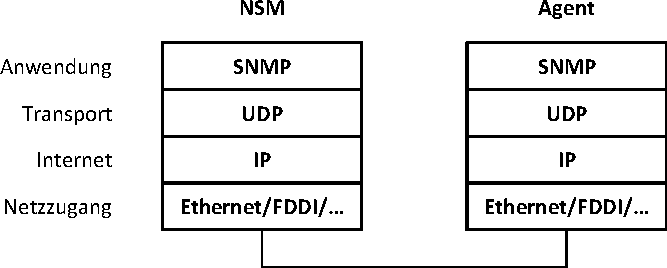
\includegraphics{bilder/tcpipstack}
	\caption{Einordnung von SNMP im TCP/IP-Stack}
	\label{fig:tcpipstack}
\end{figure}

Standardmäßig empfängt ein Agent Anfragen auf UDP-Port 161 und versendet
Antworten zurück zum Quell-Port; Traps werden auf UDP-Port 162 versendet. Sowohl
Timeout als auch der UDP-Port (Standard 161) können in Cacti festgelegt werden.

\textbf{Communitys}\\[1ex]
In den Versionen SNMPv1 und SNMPv2 erfüllen Communitys den gleichen Zweck wie
Passwörter. Empfängt ein Agent eine Anfrage mit einer ihm unbekannten Community,
wird er auf die Anfrage nicht reagieren; empfängt eine NSM einen Trap mit einer
ihr unbekannten Community, wird sie den Trap verwerfen. Ein Agent definiert dazu
drei Communitys: 1) \enquote{Read-Only}, 2) \enquote{Read-Write} und 3)
\enquote{Trap}. Wie die Namen bereits vermuten lassen, ist 1) für den
Lesezugriff (Get-Anfragen), 2) für den Lese- und Schreibzugriff (Get- und
Set-Anfragen) sowie 3) für das Versenden von Traps zuständig. Typischerweise
werden 1) und 2) auf \enquote{\texttt{public}} bzw. \enquote{\texttt{private}}
gesetzt.

An dieser Stelle sei darauf hingewiesen, dass eine Community im Klartext
übertragen wird. Es besteht daher die Gefahr, dass ein Dritter Pakete
mitliest, und aus dem Paket-Header die Community ermittelt. %Erst mit SNMPv3
%sind weitere Maßnahmen gegen Manipulation Dritter hinzugekommen.

%In Cacti kann die Read-Community für die Messdatenerfassung festgelegt
%werden.

\subsection{Abfrage eines Managed-Objects}
Für die Abfrage eines Managed-Objects bietet Cacti bereits eine generische
Data-Input-Method namens \enquote{Get SNMP Data} mit Input-Type \enquote{SNMP}
an. Sie fragt mittels \texttt{GetRequest} ein Managed-Object zu einer gegebenen
OID ab. Durch Anlegen einer Data-Source mit \enquote{Get SNMP Data} werden die
zugehörigen Input-Fields der Data-Input-Method sichtbar, wie in Abbildung
\ref{fig:getsnmpdata} dargestellt.

\begin{figure}[ht]
	\centering
	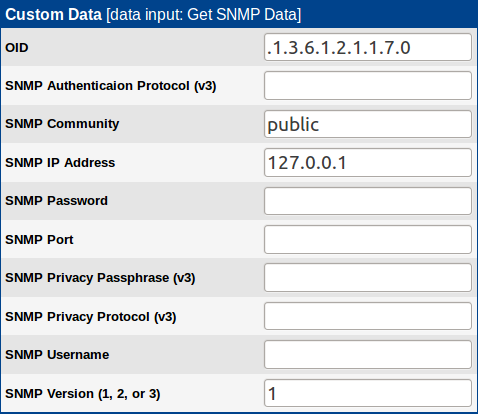
\includegraphics[scale=0.5]{bilder/getsnmpdata}
	\caption{Input-Fields von \enquote{Get SNMP Data}}
	\label{fig:getsnmpdata}
\end{figure}

Wichtig sind die Input-Fields 1) \enquote{OID}, 2) \enquote{SNMP Community}, 3)
\enquote{SNMP IP Address} und 4) \enquote{SNMP Port}. Ihnen werden 1) die OID
des abzufragenden Managed-Objects, 2) die Community für den Lesezugriff
(Standard \enquote{public}), 3) die IP-Adresse des SNMP-Agents und 4) der
UDP-Port des Agents für den Empfang von Anfragen (Standard 161) übergeben.

\subsection{Abfrage von Tabellen}
\label{subsubsec:SNMPTabelle}
Im Gegensatz zu Data-Input-Methods werden Data-Querys für die Abfrage von
indexbasierten Listen/Tabellen genutzt. Eingesetzt werden Data-Querys bspw. bei
der Abfrage von Netzwerkkarten eines Switchs, oder von Partitionen eines
File-Servers, wie in folgender Tabelle:

\begin{lstlisting}[xleftmargin=20pt]
Index  Descr            AllocationUnits  Size      Used
------------------------------------------------------------
1      C:\              4096             20479999  12520394
2      D:\              4096             57636351  9515705
3      E:\              0                0         0
4      F:\              0                0         0
5      Virtual Memory   65536            129919    57153
6      Physical Memory  65536            64974     50965
\end{lstlisting}

Dabei ist \enquote{AllocationUnits} die Blockgröße in Byte, \enquote{Size} der
verfügbare und \enquote{Used} der verwendete Speicherblatz in Blöcken. Über
SNMP lässt sich diese Tabelle abfragen. Die Werte befinden sich dazu im Teilbaum
von \\ \texttt{.1.3.6.1.2.1.25.2.3.1}.

Konfiguriert werden Data-Querys über eine XML-Datei, die das Schema der Tabelle
festlegt. Sie hat folgenden Aufbau:
\begin{lstlisting}[xleftmargin=20pt]
<query>
  <name>Get SNMP Storage Areas</name>
  <description>Liste von Partitionen<description>
  <oid_index>.1.3.6.1.2.1.25.2.3.1.1</oid_index>
  <index_order_type>numeric</index_order_type>
  <fields>...</fields>
</query>
\end{lstlisting}
Im Element \texttt{oid\_index} ist die OID anzugeben, mit der die Indizes der
Tabellenzeilen abgefragt werden. Die Sortierung der Zeilen kann bezüglich des
Index entweder numerisch  (\texttt{index\_order\_type = numeric}) oder \\
alphabetisch (\texttt{index\_order\_type = alphabetic}) erfolgen.

Die Spalten werden im Element \texttt{fields} festgelegt:
\begin{lstlisting}[xleftmargin=20pt]
<fields>
  <hrStorageDescr>
    <name>Description</name>
    <method>walk</method>
    <source>value</source>
    <direction>input</direction>
    <oid>.1.3.6.1.2.1.25.2.3.1.3</oid>
  </hrStorageDesr>
  ...
</fields>
\end{lstlisting}
Interessant sind hier die zwei Elemente \texttt{direction} und \texttt{oid}.
Ersteres kann entweder auf \enquote{\texttt{input}} oder
\enquote{\texttt{output}} gesetzt werden. Input-Spalten werden dem Nutzer für
die Auswahl der Tabellenzeilen angezeigt, bspw. wenn er eine bestimmte Partition
überwachen möchte; Output-Spalten hingegen sind die Werte, die in einem Graphen
dargestellt werden können, bspw. \enquote{Size} und \enquote{Used}. Im zweiten
Element \texttt{oid} ist die zur Spalte zugehörige OID anzugeben. 

Per \texttt{GetNext} fragt Cacti die Werte zeilenweise für jede Spalte ab. Zur
Veranschaulichung soll hier die Spalte \enquote{Descr} mit dem Werkzeug
\enquote{net-snmp} abgefragt werden:
\begin{lstlisting}[xleftmargin=20pt]
snmpgetnext -On -c public -v 2c localhost .1.3.6.1.2.1.25.2.3.1.3
> .1.3.6.1.2.1.25.2.3.1.3.1 = STRING: C:\
snmpgetnext -On -c public -v 2c localhost .1.3.6.1.2.1.25.2.3.1.3.1
> .1.3.6.1.2.1.25.2.3.1.3.2 = STRING: D:\
...
snmpgetnext -On -c public -v 2c localhost .1.3.6.1.2.1.25.2.3.1.3.5
> .1.3.6.1.2.1.25.2.3.1.3.6 = STRING: Physical Memory
\end{lstlisting}
Wobei hier die Community auf \enquote{public} und die Version auf v2 (SNMPv2)
gesetzt wurde.

Nach Anlegen einer Data-Query kann der Benutzer für jede Zeile (hier Partition)
eine Data-Source anlegen, zu jeder gewünschten Output-Spalte ein
Data-Source-Item hinzufügen und diese zur Visualisierung Graph-Items zuordnen.
Letztlich ist es damit möglich, jede Partition einzeln in einem Graph zu
überwachen.

\chapter{Messdatenspeicherung}
\label{sec:messdatenspeicherung}
Die mittels Data-Input-Methods und Data-Querys erfassten Messwerte können mit
Cacti über lange Zeiträume gespeichert und visualisiert werden. Für beide
Aufgaben nutzt Cacti das RRDTool. Hinsichtlich der Messdatenspeicherung bietet
RRDTool den Vorteil, dass der Speicherplatz stets Konstant bleibt. Der
Kompromiss dabei ist, dass viele ältere Messwerte zu wenigen konsolidierten
Messwerten zusammengefasst werden. Auf welche Weise das geschieht, wird im
nächsten Abschnitt erläutert.

\section{RRDTool-Grundlagen}
Ein Ringpuffer ist eine Speicherstruktur mit fester Größe. Es steht eine feste
Anzahl an Speicherplätzen bzw. Elementen zur Verfügung. Diese Elemente sind wie
in einem Array benachbart. Im Unterschied zum Array sind auch das erste und das
letzte Element benachbart, sodass eine Ringstruktur entsteht. Ein Pointer zeigt
auf das aktuelle Element und wird zum Schreiben um je eine Position weiter
verrückt. Zeigt der Pointer auf das letzte Element, wird er wieder auf das erste
Element gesetzt. In Konsequenz wird (nach einem Pufferüberlauf) der jeweils
älteste Wert durch den neusten Wert überschieben.

Dieses Prinzip wendet RRDTool bei der Speicherung der Messwerte in sogenannten
\enquote{Round-Robin-Archiven} (RRAs) an. In Abbildung \ref{fig:roundrobina} ist
ein RRA mit sechs Datenpunkten veranschaulicht. Um 01:01 Uhr wurde der erste
Messwert $6,1$ eingetragen, um 01:02 Uhr der zweite Messwert $4,2$ usw.;
insgesamt wurden sechs Messwerte eingetragen. Der Pointer zeigt auf den letzten
Eintrag, d.\,h. der Puffer ist voll. In \ref{fig:roundrobinb} ist der Zustand
dargestellt, nach dem der siebte Messwert $3,9$ um 01:07 Uhr hinzugefügt wurde.
Es ist zu erkennen, dass der älteste Messwert (um 01:01 Uhr) durch den neusten
(um 01:07 Uhr) überschrieben wurde.

\begin{figure}[ht]
  \centering
  \subfloat[Puffer ist voll]{
    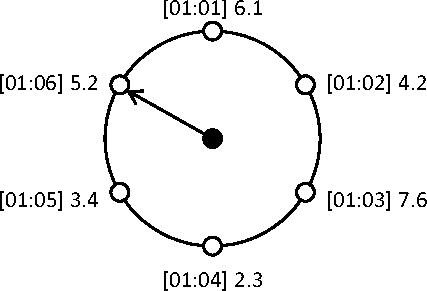
\includegraphics[width=6.0cm]{bilder/roundrobina}
    \label{fig:roundrobina}
  }
  \subfloat[Pufferüberlauf]{
    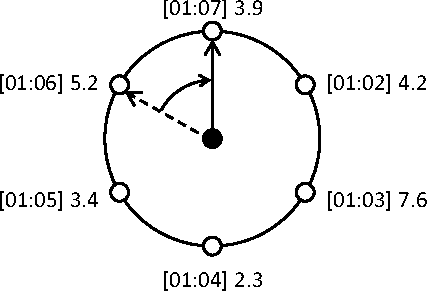
\includegraphics[width=6.0cm]{bilder/roundrobinb}
    \label{fig:roundrobinb}
  }
  \caption[Ringpufferstruktur eines RRAs]{Ringpufferstruktur eines RRAs.
  Angelehnt an \cite{Schilli04}}
  \label{fig:roundrobin}
\end{figure}

Das RRA in Abbildung \ref{fig:roundrobin} speichert die Messwerte der letzten
sechs Minuten in einer Zeitauflösung von einer Minute ab. Ist man an einem
größeren Zeitraum, bspw. einer Stunde interessiert, muss nicht die Größe des
RRAs erhöht werden. Stattdessen ist ein weiteres RRA hinzuzufügen, sodass
bspw. zehn Datenpunkte mit einer Zeitauflösung von sechs Minuten gespeichert
werden. Je sechs Datenpunkte aus dem ersten RRA werden damit zu einem Datenpunkt
des zweiten RRAs zusammengefasst, bspw. in dem der Durchschnitt oder das Maximum
gebildet wird. Durch Hinzufügen weiterer RRAs ließen sich so die Messwerte über
Tage, Monate usw. ablegen. Da jedes RRA eine feste Anzahl an Datenpunkten
besitzt, ist der benötigte Speicherplatz stets konstant. Der Kompromiss dabei
ist, dass ältere Messwerte nicht in der Zeitauflösung verfügbar sind, wie
aktuelle.

Das obige Beispiel zeigt nur das Speicherverhalten für \textit{eine}
Messgröße, tatsächlich können in einem RRA auch Werte für \textit{mehrere}
Messgrößen gespeichert werden, bspw. für die Anzahl empfangener und gesendeter
Byte einer Netzwerkkarte. Diese Messgrößen werden bei RRDTool als
\enquote{Data-Sources} (DS) bezeichnet. Für jede DS verwaltet RRDTool je ein
Ringpuffer pro RRA (Anzahl der Datenpunkte sowie Zeitauflösung bleibt pro RRA
identisch).\\
An dieser Stelle sei auf die unterschiedliche Begriffsbelegung von
\enquote{Data-Source} in Cacti und RRDTool hingewiesen. Im Bezug auf Cacti wird
daher im weiteren Verlauf \enquote{Data-Source} ausgeschrieben; im Bezug auf
RRDTool die dort gebräuchliche Abkürzung \enquote{DS} verwendet.

Zusammengefasst werden DS und zugehörige RRAs zu
\enquote{Round-Robin-Da\-ten\-bank\-en} (RRDs). RRDTool verwaltet sie in Form
von Dateien. Im Allgemeinen sind sie an der Dateiendung \enquote{.rrd} zu
erkennen. Zur Definition einer RRD gehören neben den Angaben zu DS und RRAs
auch die zwei Parameter \enquote{Start-Time} und \enquote{Step}. Messwerte, die
älter sind als die Start-Time (Angabe in Sekunden), werden ignoriert. Der
Parameter Step gibt den erwarteten zeitlichen Abstand (in Sekunden) zwischen
zwei Messwerten an. Wird er unterschritten, werden die Messwerte zu einem
Durchschnittswert zusammengefasst; wird er überschritten, werden Zwischenwerte
aus dem letzten und aktuellen Messwert interpoliert.

\subsection{Data-Source}
Eine RRD kann Messwerte aus mehreren DS aufnehmen, bspw. die Anzahl empfangener
und gesendeter Byte einer Netzwerkkarte. Innerhalb der RRD werden DS über ihren
Namen identifiziert. Weitere Parameter sind \enquote{Min-} sowie
\enquote{Max-Value}, \enquote{Data-Source-Type} (DST) und \enquote{Heartbeat}.

Min- und Max-Value legen den kleinsten bzw. größten gültigen Wert fest. Werden
diese von einem Messwert unterschritten bzw. überschritten, wird er als
\enquote{UNKNOWN}, d.\,h. als \enquote{ungültig}, in das RRA eingetragen.\\
Die Wahl des DSTs hängt von der Art der Messgröße ab, bspw. ob es sich um eine
kontinuierlich wachsende Größe handelt. In Cacti stehen vier DSTs zur Auswahl:
\enquote{GAUGE}, \enquote{COUNTER}, \enquote{DERIVE} und \enquote{ABSOLUTE}. Sie
unterscheiden sich dahingehend, wie der übergebene Messwert in ein RRA
eingetragen wird. Seien $(t_l, v_l)$, $(t_n, v_n)$ die Zeitpunkt-Messwert-Paare
der letzten bzw. aktuellen Messung, wobei $t_l$ und $t_n$ in Sekunden angegeben
sind. Der eingetragene Messwert $v_u$ berechnet sich schließlich wie folgt:

\begin{itemize}
  \item GAUGE: $v_u = v_n$, d.\,h. der aktuelle Messwert wird direkt
  übernommen.
  \item COUNTER:
\[
v_u = \begin{cases}
 \frac{v_n - v_l + 2^{32}}{t_n - t_l}, & \text{wenn} -2^{32} \leq
(v_n - v_l) < 0\\
 \frac{v_n - v_l + 2^{64}}{t_n - t_l}, & \text{wenn} -2^{64} \leq
(v_n - v_l) < -2^{32}\\
 \frac{v_n - v_l}{t_n - t_l}, & \text{sonst}\\
\end{cases}
\]\\
Dieser DST ist für kontinuierlich wachsende Größen (Zähler) geeignet, bspw. die
Anzahl empfangener Byte. Im Normalfall gilt $v_n \geq v_l$, d.\,h. die Messgröße
ist gewachsen oder gleichgeblieben. Das Besondere an COUNTER ist die Behandlung
von Überläufen. Tritt ein Überlauf des Zählers ein, wird noch einmal ab Null begonnen
zu zählen, daher gilt $v_n - v_l < 0$. Die ersten beiden Fälle der
Fallunterscheidung behandeln den Überlauf eines 32-Bit bzw. 64-Bit Zählers, der
letzte Fall entspricht dem Normalfall (der Wert ist gestiegen oder
gleich geblieben).
  \item DERIVE: $v_u = \frac{v_n - v_l}{t_n - t_l}$, wie COUNTER jedoch
  ohne Überlaufbehandlung.
  \item ABSOLUTE: $v_u = \frac{v_n}{t_n - t_l}$, ist geeignet für Zählgrößen,
  die während der Messung auf Null zurück gesetzt werden.
\end{itemize}

Wie oben angegeben, erwartet RRDTool die Messwerte in einem gewissen
Zeitabstand, der durch den Parameter Step angegeben wird. Mit dem Parameter
Heartbeat wird festgelegt, in welchem Zeitabstand höchstens zwei Messungen
auseinander liegen dürfen, bis die aktuelle als ungültig markiert wird.
Bei einer späteren Datenabfrage wird angenommen, dass die Messwerte
im Zeitabstand Step eingetragen wurden.

\subsection{Round-Robin-Archive}
Ein RRA besteht aus mehreren Ringpuffern (für jede DS einer). Darin werden die
Messdaten mit gleicher Zeitauflösung gehalten. Die größte wählbare
Zeitauflösung, d.\,h. der kleinste Zeitabstand, gibt die übergeordnete RRD
mit dem Parameter Step an. Messdaten, die ggf. zusammengefasst (Zeitabstand war
kleiner als Step) oder interpoliert (Zeitabstand war größer als Step) wurden,
werden als \enquote{Primary-Data-Points} (PDPs) bezeichnet. Pro RRA muss durch
den Parameter \enquote{Steps} angegeben werden, wie viele PDPs zu einem
\enquote{Consolidated-Data-Point} (CDP) zusammengefasst werden. Diese CDPs sind
die Einträge in den Ringpuffern.\\
Insgesamt gehören folgende Parameter zur Definition eines RRAs: \enquote{Rows}, \\
\enquote{Steps}, \enquote{Consolidation-Function} (CF) und
\enquote{X-Files-Factor} (XFF).
Ein Ringpuffer speichert eine feste Anzahl an Elementen (hier CDPs) ab. Die
Anzahl an CDPs legt der Parameter Rows fest. Werden mehr CDPs in einem
Ringpuffer abgelegt, als in Rows angegeben, werden ältere Einträge durch neuere
überschrieben.\\
Steps legt fest, wie viele PDPs zu einem CDP zusammengefasst werden. Demzufolge
kann ein RRA Messdaten in einer Zeitspanne von
$\text{Step}*\text{Steps}*\text{Rows}$ Sekunden archivieren.\\
Wie die PDPs zu einem CDP zusammengefasst (konsolidiert) werden, legt die CF
fest. Folgende vier CFs werden angeboten:
\begin{enumerate}
  \item MIN: $\text{CDP} = \min(\text{PDP}_1, \text{PDP}_2, \ldots,
  \text{PDP}_{\text{Steps}})$, d.\,h. der \textit{kleinste} PDP wird ausgewählt.
  \item MAX: $\text{CDP} = \max(\text{PDP}_1, \text{PDP}_2, \ldots,
  \text{PDP}_{\text{Steps}})$, d.\,h. der \textit{größte} PDP wird ausgewählt.
  \item LAST: $\text{CDP} = \text{PDP}_{\text{Steps}}$, d.\,h. der
  \textit{letzte} PDP wird ausgewählt.
  \item AVERAGE: $\text{CDP} =
  \frac{1}{\text{Steps}}\sum\limits_{i=1}^\text{Steps} \text{PDP}_i$, d.\,h. es
  wird der Durchschnittswert aus allen PDPs berechnet.
\end{enumerate}
Während der Messung können mehrere PDPs als ungültig gespeichert wurden sein,
bspw. weil der Min- oder Max-Value unter- bzw. überschritten wurde. Der
Parameter $\text{XFF} \in [0, 1)$ gibt das maximale Verhältnis von ungültigen zu
gültigen PDPs an. Wird es unterschritten, wird der CDP selber als ungültig
gespeichert.

\textbf{Beispiel}\quad Eine RRD mit zwei RRAs:\\[1ex]
Zur Veranschaulichung ist in Abbildung \ref{fig:rra} eine Beispiel-RRD
mit Step = \mbox{60 s}, sechs Messwerten und zwei RRAs angegeben. Im oberen
Bereich wird gezeigt, wie die Messwerte auf PDPs abgebildet werden. Der Messwert zum
Zeitpunkt 90 s hat zum vorhergehenden Messwert nur 30 s Abstand und
unterschreitet damit den Step-Wert von 60 s. Daher wird er mit dem nächsten
Messwert (Zeitpunkt 120 s) zum PDP $3 = \frac{1 + 5}{2}$ zusammengefasst. Alle
weiteren Messwerte haben einen Abstand von 60 s und können damit direkt auf PDPs
abgebildet werden.\\
Das erste RRA speichert Rows = 5 CDPs. Da Steps = 1 gesetzt wurde, wurden die
PDPs direkt auf die CDPs abgebildet. Mit 5 CDPs ist der Ringpuffer voll. Jeder
weitere Eintrag eines CDPs würde ältere CDPs überschreiben.\\
Beim zweiten RRA wird die CF = AVERAGE benötigt. Es werden jeweils aus Steps = 5
PDPs ein CDP gebildet, in dem der Durchschnitt berechnet wird. Hier ergibt sich
der erste CDP $5,8$ aus $\frac{4 + 3 + 6 + 9 + 7}{5}$. Alle vier weiteren CDPs
im RRA sind noch nicht belegt, und daher auf \enquote{Not a Number}(dt.
\enquote{keine Zahl}, NaN) gesetzt.

\begin{figure}[ht]
	\centering
	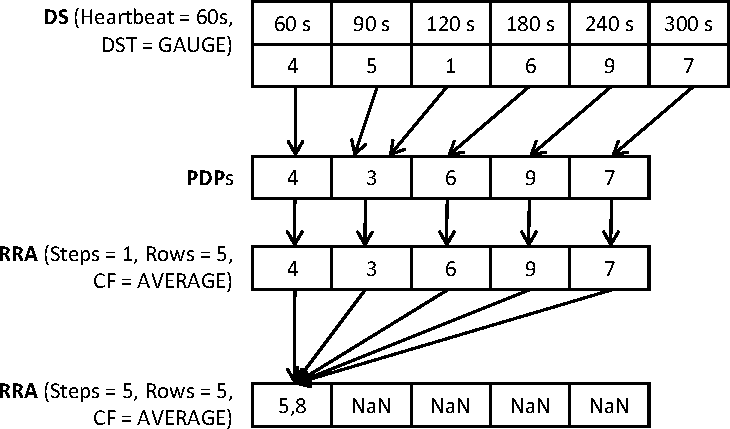
\includegraphics[scale=0.9]{bilder/rra}
	\caption{Beispiel-RRD mit zwei RRAs und Step = 60 s}
	\label{fig:rra}
\end{figure}

\section{Zusammenhang zwischen RRDTool und Cacti}
Die Unterteilung in DS und RRAs findet sich in Cacti wieder; jedoch unter
anderen Begriffen. Was in RRDTool mit RRD bezeichnet wird, heißt in Cacti
Data-Source. Daher ist jeder Data-Source eine RRD-Datei zugeordnet. Eine
Data-Source ist beschränkt auf eine Data-Input-Method, d.\,h. es können nicht
Messwerte aus unterschiedlichen Data-Input-Methods gespeichert werden. Jede
Data-Input-Method besitzt mindestens ein Output-Field. Zur Speicherung der
Messwerte eines jeden Output-Fields ist ein zugehöriger Data-Source-Item in der
Data-Source anzulegen. Ein Data-Source-Item entspricht einer DS in RRDTool. Die
zugehörigen Parameter für Data-Source und Data-Source-Item sind in Abbildung
\ref{fig:datasourcea} bzw. \ref{fig:datasourceb} dargestellt.

\begin{figure}[ht]
  \centering
  \subfloat[Data-Source]{
    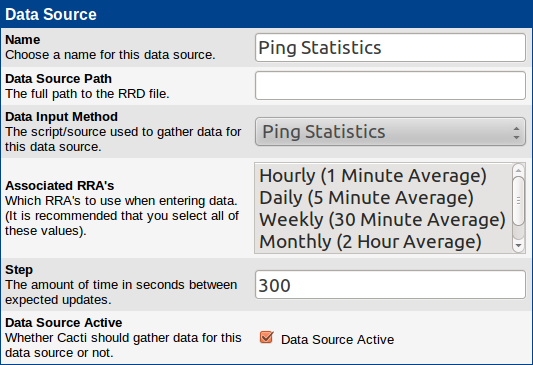
\includegraphics[width=6.5cm]{bilder/datasourcea}
    \label{fig:datasourcea}
  }
  \subfloat[Data-Source-Item]{
    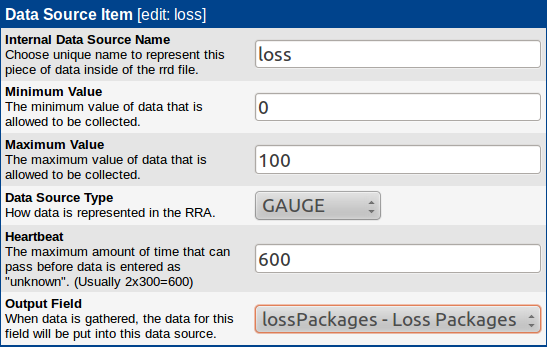
\includegraphics[width=6.5cm]{bilder/datasourceb}
    \label{fig:datasourceb}
  }
  \caption{Parameter von Data-Source und Data-Source-Item}
  \label{fig:datasource}
\end{figure}

Bei \enquote{Data-Source-Path} wird der Pfad zur RRD-Datei angegeben. Der
Parameter \enquote{Internal-Data-Source-Name} gibt den Namen der RRDTool-DS an.
Auch weitere Parameter finden ihre Entsprechung in RRDTool:
\begin{itemize}
  \item Associated-RRAs: Entspricht den RRA-Definitionen in einer RRD. Die von
  Cacti angebotenen RRAs haben den DST = AVERAGE. Jedoch lassen sich weitere
  RRA-Vorgaben mit anderen Steps-, Rows- und CF-Argumenten anlegen.
  \item Step: Entspricht dem Step-Parameter in einer RRD.
  \item Minimum- und Maxmimum-Value: Entspricht den Parametern Min- und
  Max-Value einer DS in RRDTool.
  \item Data-Source-Type: Entspricht dem DST-Parameter einer DS.
  \item Heartbeat: Entspricht dem Heartbeat-Parameter einer DS.
\end{itemize}

\chapter{Messdatendarstellung}
Neben der Messdatenspeicherung setzt Cacti auch bei der Messdatendarstellung auf
RRDTool. In regelmäßigen Abständen werden Diagramme -- in Cacti als
\enquote{Graphs} bezeichnet -- mit RRDTool erstellt und auf der Weboberfläche
dargestellt. Als Bildformate werden \enquote{Portable Network Graphics} (PNG),
\enquote{Graphics Interchange Format} (GIF) und das Vektorgrafikformat
\enquote{Scalable Vector Graphics} (SVG) angeboten. Bei der Erstellung eines
Graphs können u.\,a. folgende Parameter angegeben werden:
\begin{itemize}
  \item Title: Titel-Text, der oberhalb des Graphs positioniert wird.
  \item Vertical-Label: Vertikal platzierter Text auf der linken Seite des
  Graphs.
  \item Width und Height: Breite und Höhe des Graphs in Pixel.
  \item Skalierung der Y-Achse: Entweder skaliert RRDTool die Y-Achse
  automatisch oder man gibt eine untere (Lower-Limit) und/oder obere Grenze
  (Upper-Limit) an. Desweiteren ist eine logarithmische Skalierung der Y-Werte
  möglich.
\end{itemize}
Die Messwerte können als Linien- oder Flächendiagramme dargestellt werden. Jede
einzuzeichnende Komponente ist als sogenannter \enquote{Graph-Item} dem Graph
hinzuzufügen. Dazu gehört bspw. \enquote{LINE}, der Datenpunkte durch eine
Linie verbindet (Liniendiagramm). Darüber hinaus ist es möglich, Funktionen
auf Datenpunkte anzuwenden. Das wird nötig, wenn bspw. die
Übertragungsgeschwindigkeit in Byte/s gegeben ist und im Graph in Bit/s
dargestellt werden soll. Hier müssen die Werte erst mit 8 multipliziert werden.
Für diese und weitere Berechnungen bietet RRDTool die sogenannten
\enquote{CDEF-Anweisungen}. Diese führen Berechnungen elementweise auf
einer Werteliste aus und weisen das Ergebnis neuen Variablen zu.

In den Abschnitten \ref{subsec:GraphItems} und \ref{subsec:CDEF}
werden Graph-Items und CDEF-Anweisungen vorgestellt.

\section{Graph-Items}
\label{subsec:GraphItems}
Obwohl Cacti auf Linien- und Flächendiagramme begrenzt ist, bleibt die
Gestaltung eines Graphs durch die Kombinationsmöglichkeiten verschiedener
Graph-Items flexibel. Graph-Items sind Graphs untergeordnet und modellieren
darzustellende Komponenten im Graph. Zu den angebotenen Graph-Item-Typen gehören
u.\,a.:
\begin{itemize}
  \item LINE: Die Datenpunkte eines Data"-Source"-Items bzw. einer CDEF"-Variablen
  werden durch eine Linie verbunden (Liniendiagramm). Es kann festgelegt
  werden, mit welcher Farbe und welcher Dicke (1, 2, oder 3 Pixel) die Linie zu
  zeichnen ist. Cacti erstellt automatisch einen Eintrag mit Linienfarbe und
  Text in der Legende des Graphs. 
  \item AREA: Die Fläche zwischen den verbundenen Datenpunkten und der X-Achse
  wird gefüllt (Flächendiagramm). Auch hier lässt sich die Flächenfarbe angeben
  und es wird ein Eintrag in der Legende erstellt.
  \item HRULE: Zu einem festen Y-Wert wird eine horizontale Linie eingezeichnet.
  Diese kann bspw. einen kritischen Schwellwert (maximale Festplattenauslastung
  u.\,ä.) darstellen.
  \item VRULE: Zu einem festen X-Wert wird eine vertikale Linie eingezeichnet.
  \item GRPINT: Expliziter Eintrag in der Legende, um den größten, kleinsten,
  letzten Wert oder den Durchschnittswert eines Data"-Source"-Items bzw. einer
  CDEF-Variablen im Graph zu vermerken.
\end{itemize}
Durch Kombination aus zwei LINE-Graph-Items ist es bspw. möglich, die Sende-
und Empfangsgeschwindigkeit einer Netzwerkkarte in einem Graph mit
unterschiedlichen Farben darzustellen.

\section{Berechnungen mittels CDEF-Anweisungen}
\label{subsec:CDEF}
CDEF-Anweisungen sind mathematische Funktionen, die auf Messwerte elementweise
angewandt werden. Das Ergebnis wird in einer Variablen gespeichert. Über den
Namen der Variablen kann die neu berechnete Datenreihe in den Graph gezeichnet
oder erneut als Argument einer anderen CDEF-Anweisung übergeben werden. Der
Berechnungsausdruck wird in der \enquote{Umgekehrt Polnischen Notation} (engl.
Reverse Polish Notation, kurz RPN) angegeben. Als Rechenmodell dient hier eine
Stackmaschine. Auf den Stack sind zunächst die Operanden abzulegen (Push). Beim
Ausführen einer Operation werden die Operanden vom Stack geholt (Pop), die
Berechnung durchgeführt und das Ergebnis auf den Stack gelegt (Push). Beispiel:
Der Infix-Ausdruck $3+4*5$ (Operator steht zw. den Operanden) ist äquivalent zum
RPN-Ausdruck \texttt{4,5,*,3,+} (Operator steht hinter den Operanden).

In Cacti werden diese CDEF-Anweisungen separat von den Graphs verwaltet. Zur
Definition einer CDEF-Anweisung gehören ein eindeutiger Name sowie ein oder
mehrere \enquote{CDEF-Items}. Diese CDEF-Items modellieren die Operanden bzw.
Operatoren des RPN-Ausdrucks. Daher ist deren Reihenfolge zu beachten.

\textbf{Beispiel}\quad Umrechnung von Byte/s in Bit/s\\[1ex]
Angenommen die Übertragungsgeschwindigkeit einer Netzwerkkarte wird in
Byte/s gemessen, soll jedoch in Bit/s angezeigt werden. Dafür ist eine
CDEF-Anweisung mit den folgenden CDEF-Items zu erstellen:
\begin{enumerate}
  \item CURRENT\_DATA\_SOURCE: CDEF-Anweisungen werden getrennt von Graphs
  verwaltet. Bei der Definition einer CDEF-Anweisung ist daher nicht bekannt,
  auf welchem Data"-Source"-Item die Berechnung durchgeführt
  werden soll. Bei \enquote{CURRENT\_DATA\_SOURCE} ersetzt Cacti
  automatisch diesen CDEF-Item durch den in einem Graph-Item angegebenen
  Data-Source-Item.
  \item Custom String \enquote{8}: Operand \enquote{8} für die Multiplikation,
  um Byte in Bit umzurechnen.
  \item Operator \enquote{*}: Multiplikation mit der 8.
\end{enumerate}
Letztlich wird damit der RPN-Ausdruck
\enquote{\texttt{CURRENT\_DATA\_SOURCE,8,*}} beschrieben, der auf jeden Messwert
angewandt wird.

Zu den arithmetischen Operatoren werden auch boolesche Operatoren,
trigonometrische Operatoren, Mengenoperatoren und weitere angeboten. Alle
Berechnungen auf den Datenpunkten werden unabhängig voneinander durchgeführt.

\textbf{Beispiel}\quad Farbiges hervorheben kritischer Übertragungsraten\\[1ex]
Ein Mittel, um auf kritische Werte hinzuweisen, ist das farbige Hervorheben
dieser. Beispielsweise können \enquote{optimale} Werte grün, normale Werte gelb
und kritische Werte rot dargestellt werden. Sei $r$ eine
gemessene Übertragungsrate. Im Beispiel sollen Werte $r > 350
\text{kBit/s}$ dem optimalen Bereich, Werte $100 \text{kBit/s} < r \leq 350
\text{kBit/s}$ dem normalen Bereich und Werte $r \leq 100 \text{kBit/s}$ dem
kritischen Bereich zugeordnet werden.

Generell ist das Zeichnen mehrfarbiger LINE- bzw. AREA-Graph-Items nicht
möglich. Für die Umsetzung können jedoch mehrere Graph-Items
unterschiedlicher Farbe miteinander kombiniert werden. Die Idee ist, Werte
außerhalb eines Bereichs zu Null zu setzen. Dazu werden folgende drei
CDEF-Anweisungen definiert:
\begin{lstlisting}[xleftmargin=20pt]
optimal = CURRENT_DATA_SOURCE,350000,GT,
  CURRENT_DATA_SOURCE,0,IF
normal = CURRENT_DATA_SOURCE,350000,LE,CURRENT_DATA_SOURCE,
  100000,GT,1,EQ,EQ,CURRENT_DATA_SOURCE,0,IF
kritisch = CURRENT_DATA_SOURCE,100000,LE,
  CURRENT_DATA_SOURCE,0,IF
\end{lstlisting}
Der RPN-Ausdruck für die CDEF-Variable \enquote{normal} ist wie folgt zu lesen:
\begin{enumerate}
  \item Lege aktuellen Messwert und 350000 auf den Stack und vergleiche beide
  mittels \enquote{LE-Operator} (engl. \enquote{lower or equal}). Dieser liest
  zwei Werte $a,b$ und legt eine Eins auf den Stack, wenn $a \leq b$ gilt; sonst
  eine Null.
  \item Analog ist \enquote{\texttt{CURRENT\_DATA\_SOURCE,100000,GT}} zu lesen,
  wobei GT (engl. \enquote{greater than}) auf $a>b$ prüft.
  \item Mittels \texttt{1,EQ,EQ} wird eine Eins auf den Stack gelegt, wenn beide
  Bedingungen erfüllt sind; sonst eine Null. Dabei prüft \enquote{EQ} auf $a=b$.
  \item Der \enquote{IF-Operator} stellt einen bedingten Ausdruck dar. Es gilt
  bei \texttt{A,B,C,IF}: Wenn $A = 1$ wird B, sonst C auf den Stack gelegt.
  Erfüllt hier der Messwert beide Bedingungen, wird er auf den Stack gelegt;
  sonst eine Null.
\end{enumerate}
Für jede CDEF-Anweisung wird ein AREA-Graph-Item erstellt, und ihm grün für
\enquote{optimal}, gelb für \enquote{normal} und rot für \enquote{kritisch}
zugewiesen. In Abbildung \ref{fig:cdef} ist dieses Verhalten dargestellt.

\begin{figure}
	\centering
	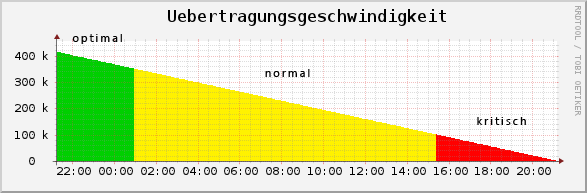
\includegraphics[scale=0.5]{bilder/cdef}
	\caption{Mehrfarbiges Flächendiagramm}
	\label{fig:cdef}
\end{figure}

\chapter{Anwendungsbeispiel: Privater Homeserver}
\label{sec:Anwendungsbeispiel}
In diesem Kapitel soll der praktische Einsatz von Cacti anhand eines privaten
Homeservers gezeigt werden. Über Systemprogramme lassen sich Hardwareressourcen,
wie RAM-Verbrauch und Prozessorauslastung, abfragen. Auch Serverdienste, wie
HTTP und FTP, stellen ihre Metriken typischerweise in Form von Log-Dateien zur
Verfügung. Cacti ermöglicht es hier, diese Hardwareressourcen und Metriken
zentral und einheitlich über eine Weboberfläche zu überwachen. Im Abschnitt
\ref{subsec:Konfiguration} wird die Konfiguration des betrachteten Homeservers
und im Abschnitt \ref{subsec:Anwendungsbeispiele} Anwendungsbeispiele von
Cacti beim Überwachen des Homeservers beschrieben.

\section{Konfiguration des Homeservers}
\label{subsec:Konfiguration}
Als Betriebssystem ist Linux auf dem Homeserver installiert. Gesichert wird der
Homeserver über die Linux-eigene Firewall \enquote{iptables}. Installiert wurden
verschiedene Server-Anwendungen. Dazu zählen der Apache2-Webserver, das
OpenSSH-Programmpaket für die Unterstützung von SSH, ein FTP-Server, ein
E-Mail-Server mit IMAP-Unterstützung, der Instant-Messenger-Server Jabberd2 und
ein Ventrilo-Server zum Anbieten von Internet-Telefonie.

Zusätzlich werden weitere Programme für die Installation von Cacti
vorausgesetzt: Cacti wurde zu einem Großteil in PHP entwickelt, weswegen ein
entsprechender PHP-Interpreter benötigt wird. Ein MySQL-Server wird
vorausgesetzt, um Einstellungen in Form von Tabellen zu speichern. Für die
Messdatenspeicherung und -Visualisierung wird das RRDTool benötigt.

\section{Anwendungsbeispiele von Cacti}
\label{subsec:Anwendungsbeispiele}
In diesem Abschnitt werden Anwendungsbeispiele beschrieben, bei denen Cacti für
das Monitoring des Homeservers eingesetzt wird. Alle Anwendungsbeispiele haben
gemeinsam, dass die zu überwachenden Metriken aus Log-Dateien ermittelt werden
können. Die Formate der Log-Dateien unterscheiden sich von Software zu Software.
Cacti erwartet die Messwerte in einem bestimmten Format, wie in Abschnitt
\ref{subsec:AbfrageScript} beschrieben. Entsprechend sind die Messdaten für
jedes Log-Datei-Format individuell in das von Cacti geforderte Format zu
überführen. Der hier gewählte Ansatz zur Messdatenerfassung verarbeitet die
Log-Dateien via Bash-Scripts. Mittels awk, grep, cat etc.
werden die relevanten Messdaten ausgelesen und Cacti im gewünschten Format
übergeben. Der Poller führt in festen Zeitintervallen diese Scripts aus und
speichert die Messdaten in den RRDs ab. Anschließend lassen sich die Messdaten
in Form von Diagrammen visualisieren.

Vorgestellt werden folgende
 Anwendungsbeispiele: Ermitteln der
Ge\-sprächs\-teil\-neh\-mer\-zahl (Ventrilo-Server), Ermitteln des Verbrauchs
eines Verzeichnisses (samt Unterverzeichnissen), die Zählung vollständiger Downloads,
die Zählung missglückter Anmeldeversuche unter SSH, die Zählung vollständiger
Downloads unter Berücksichtigung dass Logdateien archiviert werden und das
Auslesen des Onlinestatus unter Jabberd2. Jedem Anwendungsbeispiel ist ein
Bash-Script zugeordnet. Dabei sind die erforderlichen Benutzerrechte zum
Ausführen der Bash-Scripts zu beachten. Ein Anwendungsbeispiel ist untergliedert
in Überblick, Formatbeschreibung und Erläuterung zum Bash-Script.

\subsection{Ventrilo: Aktuelle Teilnehmerzahl}
Ventrilo nennen sich zwei Programme, ein Server und ein Client. Diese
Kombination wird für Internet-Telefonie in Gruppen verwendet, ohne dass
eine Anbindung an das Telefonnetz vorliegt. Alternative  Lösungen sind:
Teamspeak, Mumble/Murmur oder Skype.

Die vom Ventrilo-Server erzeugte Logdatei eignet sich zum Auswerten der
Gesprächsteilnehmeranzahl. Darin liegen die Informationen wann sich jemand zum
Server verbindet und wann jemand den Server verlässt. Es werden darin
Verbindungsdaten gelistet. So ist es möglich mit einem Skript auszuwerten, wie
viele Gesprächsteilnehmer zur Zeit in Ventrilo anwesend sind. In Cacti lässt
sich schließlich über einen längeren Zeitraum einsehen, wann wie viele Personen
auf einem Ventrilo-Server anwesend waren. Ein Auszug aus einer solchen Logdatei
ist in Listing 1 dargestellt.

\begin{lstlisting}[caption={Auszug aus einer
Ventrilo-Logdatei}\label{lst:VentriloLog},captionpos=b,numbers=left]
READY
...
READY
20160409 18:53:33 MSG_CONN: ID 423, IP 139.18.185.81, Accepted. 
20160409 20:50:45 NET: ID 423, Disconnect, 104. 
20160409 20:50:45 MSG_DISC: ID 423, From=20162, To=14079643, Sec=7032, Name=benutzer2
\end{lstlisting}

Eine Zeile in der Logdatei ist wie folgt von links nach rechts aufgebaut:
\begin{itemize}
  \item Jahr, Monat, Tag oder \enquote{Ready}. Die letzte \enquote{Ready}-Zeile
  markiert den Beginn der Zählung.
  \item Uhrzeit
  \item Tatbestand: Netzwerkmeldung/ Verbindung/ Trennung
  \item \enquote{ID}  wenn die ID des Nutzers folgt
  \item ID des Nutzers als Zahl -- Diese sind eindeutig pro Login und Logout
  \item Tatbestand Getrennt / \enquote{IP} wenn IP folgt / \enquote{From=}
  ventrilo-interne Nummer
  \item IP Adresse / Logdateizeilenart als Nummer / \enquote{To=} interne Nummer
  \item z.\,B. \enquote{Accepted} d.\,h. Reaktion des Servers /\enquote{Sec=}
  Sekunden der Anwesenheit
  \item \enquote{Name=} verwendeter Name des Nutzers im Programm 
\end{itemize}

In Listing 1 ist zu erkennen, dass zunächst 0 Nutzer
online sind. Ab der ersten Zeile des Ausschnittes ist 1 Nutzer online
(\texttt{MSG\_CONN}=verbinden). Dieser trennt sich danach vom Server und somit
sind wieder 0 Nutzer online (\texttt{Disconnect} und \texttt{MSG\_DISC}).

In Listing 2 ist der Bash-Script dargestellt, mit dem die Verbindungen ermittelt
werden. Ausgegeben wird die Anzahl an Verbindungen minus die Anzahl an Abbrüchen
minus die Anzahl an vollendeten Trennungen. Diese 3 Variablen sind relevant für
die Berechnung wie viel Nutzer aktuell mit dem Server verbunden sind. Bei einem
Neustart des Servers wird die Logdatei fortgeführt und einige Zeilen markieren
den Start des Servers in der Logdatei. Die letzte Zeile dieser Zeilen lautet
\enquote{Ready}. Ab der \enquote{Ready}-Zeile kann die Zählung beginnen.

\begin{lstlisting}[caption={Script zur Auswertung von
Ventrilo-Logdateien}\label{lst:VentriloBash},captionpos=b,numbers=left]
#!/bin/sh

beginnen=`cat /opt/ventrilo-3.0/ventrilo_srv.log | grep -n READY: | tail -1 | awk '{print $1}'`
enden=`cat /opt/ventrilo-3.0/ventrilo_srv.log | grep -n ' ' | tail -1 | awk '{print $1}'`

a=`expr index ${beginnen} ':'`
a=`expr ${a} - 1`
begin=`expr substr ${beginnen} 1 ${a}`

b=`expr index ${enden} ':'`
b=`expr ${b} - 1`
ende=`expr substr ${enden} 1 ${b}`

diff=`expr ${ende} - ${begin} + 1`

befehl=`echo 'tail ';echo -${diff} ;echo '/opt/ventrilo-3.0/ventrilo_srv.log'`

a=`${befehl} | grep Accepted | grep -c MSG_CONN`
b=`${befehl} | grep -c MSG_ABORT`
c=`${befehl} | grep -c MSG_DISC`

expr  $a - $b - $c
\end{lstlisting}

Das Script in Listing 2 arbeitet wie folgt: Es werden
Zeilennummern und Zeilen in der Logdatei mit dem Inhalt \enquote{READY:}
abgefragt (Zeile 3), davon wird die letzte Zeile verwendet und davon die
Zeichenketten vor dem ersten Whitespace. Das ist die Zeilennummer mit weiteren
Zeichenketten. Dies wird in der Variable \enquote{beginnen} gespeichert. Diese
Zeilennummer markiert den letzten Start oder Neustart des Ventriloservers.\\
Analog werden in „enden“ die letzte Zeile und die restlichen Zeichenketten der
Logdatei gespeichert (Zeile 4). In \enquote{a} wird die letzte Stelle der
Zeilennummer ermittelt (Zeile 6 und 7) und schließlich für die Variable
\enquote{begin} nur die Zeilennummer entnommen (Zeile 8). Analog wird mittels
\enquote{b} in \enquote{ende} die letzte Zeile gespeichert (Zeile 10 bis 12). In
\enquote{diff} ist die Differenz der Zeilen vom \enquote{begin} und
\enquote{ende} plus 1 gespeichert (Zeile 14).\\
Die Variable \enquote{befehl} stellt das Kommando dar, dass nur die Zeilen vom
letzten Start des Servers bis zum Ende der Logdatei ausgegeben werden (Zeile
16). Verwendet wird sie für die folgenden drei Variablen: \enquote{a}, die die
Verbindungen, \enquote{b}, die die Abbrüche und \enquote{c}, die die nicht
abgebrochenen Trennungen speichert.\\
Ausgeben wird die Anzahl der aktuell Anwesenden auf dem Server mittels
Subtraktion a-b–c (Zeile 22).

Es ist möglich in der Ventrilo-Logdatei zu sehen, wann spezielle Benutzer online
waren. Das Problem ist jedoch, dass in der Logdatei
lediglich beim Abmelden der Benutzername enthalten ist. Jedoch muss der Poller
von Cacti früher darüber informiert sein, dass eine spezielle Person anwesend
ist. Eine Variante dieses Problem zu lösen ist die Systemzeit kurzfristig
zurückzustellen, kurz bevor ein zweiter anders konfigurierter Poller aktiv wird,
der lediglich meldet, dass jemand zu einer speziellen Zeit auf den
Ventrilo-Server gekommen ist. Nachträgliche Änderungen in den RRA-Dateien
mittels RRD-Tools sind jedoch nicht möglich, so dass die Idee dahinter verworfen
werden muss. Das bedeutet, dass Cacti sich nicht für diesen Zweck eignet. In
Konsequenz können die betroffenen Personen mit Cacti nicht überprüfen, wann sie
in ihrer Vergangenheit in Ventrilo anwesend waren.

\subsection{Verbrauch eines Verzeichnisses samt Unterverzeichnissen}
Dieses Anwendungsbeispiel dient der Ermittlung von einzelnen Bereichen auf der
Festplatte, d.\,h. wie sich Verzeichnisse in der Größe ändern, um reagieren zu
können, wenn zu wenig Speicher frei ist oder um eine Übersicht über
diese Größen zu gewinnen. In Abschnitt \ref{subsubsec:SNMPTabelle} wird ein
ähnliches Beispiel betrachtet. Es ermittelt die Partitionsgrößen per SNMP. Das
Beispiel in diesem Abschnitt unterscheidet sich dazu, dass die Größe eines
einzelnen Verzeichnisses mittels Script ermittelt wird.

Da der Poller gewöhnlich über keine Administrator-Rechte verfügt, und das
Verzeichnis andere Benutzerrechte als der aktive Poller besitzt, muss die
Umsetzung erweitert werden. Ein zusätzlicher Cronjob mit entsprechenden Rechten
kann die Dateigröße als Zahl in eine Textdatei schreiben und ihr anschließend
die benötigten Rechte zuweisen, die sie für den Poller lesbar macht. Das Script
für diesen Cronjob ist in Listing 3 dargestellt. Es
speichert die Verzeichnisgröße (in Byte) in der Datei \enquote{abc.txt}. Cacti
besitzt die Rechte des Benutzers \enquote{cactiuser} und kann somit diese
erzeugte Datei auslesen.\\
Zur Messdatendarstellung eignen sich Graphen mit verschiedenen Flächen (Areas),
so dass die Größen von mehreren Ordnern der Gesamtgröße gegenübergestellt werden
können.

\begin{lstlisting}[caption={Script des Cronjobs zur Ermittlung des
Verzeichnisverbrauchs}\label{lst:VerzeichnisBash},captionpos=b,xleftmargin=20pt]
du -sb /ordner1/ordner2 2> /dev/null | awk '{print $1}' >  /ordner3/abc.txt
chmown cactiuser /ordner3/abc.txt
\end{lstlisting}

In der Abfrage von Cacti ist es nicht nötig eine Scriptdatei anzugeben. Es
genügt die Abfrage mittels \texttt{echo /ordner3/abc.txt}. 

Zum Addieren von speziellen Verzeichnissen eignet sich der Expr-Befehl:
\begin{lstlisting}[xleftmargin=20pt]
expr `cat 1.txt` + `cat 2.txt`
\end{lstlisting}

\subsection{Apache2: Vollständige Downloads}
\label{subsubsec:Apache2}
Der Apache2 ist ein weit verbreiteter Webserver. Mit Hilfe der Auswertung dessen
Logdatei ist es möglich, vollständige und unvollständige Downloads einer
angegeben Datei getrennt zu untersuchen.

In Listing 4 ist ein Auszug aus einer Apache2-Logdatei
dargestellt.

\begin{lstlisting}[caption={Auszug aus einer
Apache2-Logdatei}\label{lst:Apache2Log},captionpos=b,xleftmargin=20pt]
127.0.0.1 - - [17/Feb/2016:16:27:09 +0100]
  "GET /beispiel.dat HTTP/1.1" 200 910015423 "-"
  "Mozilla/5.0 (X11; Linux x86_64; rv:10.0)
  Gecko/20150101 Firefox/36.0" 373 140243252
\end{lstlisting}

Die dargestellte Zeile in Listing 4 ist wie folgt von links
nach rechts aufgebaut:
\begin{enumerate}
  \item IP Adresse des Browsers
  \item Datum und Uhrzeit
  \item Zeitzone
  \item Kommando des Browsers „GET“
  \item Zugriff auf Pfad mit Datei auf dem Webserver
  \item verwendete HTTP-Version
  \item Befehlsnummer
  \item Dateigröße der herunterzuladenden Datei durch den Browser
  \item Name des Browserbackends mit Version
  \item Fenstersystem
  \item Betriebssystem
  \item Architektur
  \item Version des Browserfrontends
  \item Rendering Engine des Browsers
  \item Name des Browsers mit Version
  \item Nummer der Reaktion des Webservers
  \item übertragene Bytes der herunterzuladenden Datei
\end{enumerate}

In diesem Beispiel wurden 140243252 Byte der Datei \enquote{beispiel.dat}
heruntergeladen wobei die Dateigröße 910015423 Byte beträgt. Die Differenz
beider Größen ist der Indikator dafür, ob es sich um einen vollständigen oder
unvollständigen (wie im Beispiel) Download handelt.

Das Script zum Ermitteln der vollständigen und unvollständigen Downloads für die
Datei \enquote{beispiel.dat} ist in Listing 5 dargestellt.

\begin{lstlisting}[caption={Script zum Ermitteln von vollständigen und
unvollständigen Downloads}\label{lst:Apache2Bash},captionpos=b,numbers=left]
#!/bin/bash

c=`cat /var/log/apache2/access_log | grep beispiel.dat`
a=`echo "$c"  | awk '{printf "%s \n",$10}'| sed '1q;d'`
b=`echo "$c" | awk '{print $20}'`
i1=0
i2=0

for i in `echo "$b"`
do
  c=`echo $b |  awk '{print $'$i'}'`
  if [ $i == $a ]
  then i1=`expr $i1 + 1`
  else i2=`expr $i2 + 1`
  fi
done
i3=`expr $i1 + $i2`

case "$1" in
    voll) echo $i1
    ;;
    unvoll) echo $i2
    ;;
    zus) echo $i3
    ;;
esac

exit 0
\end{lstlisting}
In der Variablen \enquote{c} werden alle Zeilen der Logdatei gespeichert, die
den Download der Datei \enquote{beispiel.dat} betreffen (Zeile 3). Anschließend
wird aus der ersten gefilterten Logzeile die Dateigröße ermittelt und in der
Variablen \enquote{a} gespeichert (Zeile 4). Analog dazu wird in \enquote{b} die
Liste aller Downloadgrößen gespeichert (Zeile 5).\\
Die Variablen \enquote{i1} und \enquote{i2} repräsentieren die Anzahl
vollständiger bzw. unvollständiger Downloads. Berechnet werden sie in der
Zählschleife (Zeile 9 bis 15). Deren Summe wird in \enquote{i3} abgelegt (Zeile
17).\\
Abhängig vom ersten Eingabeparameter wird die Anzahl vollständiger Downloads
(\enquote{voll}), unvollständiger Downloads (\enquote{unvoll}) oder die
Gesamtanzahl (\enquote{zus}) ausgegeben (Zeile 19 bis 27).

\subsection{OpenSSH: Zählen missglückter Anmeldeversuche}
Mit SSH lässt sich ein Unix/Linux über Kommandozeile fernsteuern, entfernte
graphische Anwendungen benutzen, sofern ein X-Server installiert ist und sichere
FTP-Verbindungen aufbauen.

In der Logdatei /var/log/messages befinden sich u.\,a. Meldungen des SSH-Servers
namens \enquote{sshd}, sofern nicht eine andere Logdatei dafür definiert wurde.
Ein Auszug aus einer solchen Logdatei ist in Listing 6
dargestellt. Die Anzahl an Fehlermeldungen unter allen Meldungen des SSH-Servers
entspricht der Anzahl an missglückten Anmeldeversuchen. Diese Anzahl ist die
Grundlage für die Erzeugung des Graphen in Cacti. Zusätzlich kann der Anstieg an
missglückten Anmeldeversuchen beobachtet werden, und bei einem zu hohem Anstieg
mit Hilfe des Plug-Ins \enquote{Thold} der Administrator per E-Mail darüber
benachrichtigt werden.

\begin{lstlisting}[caption={Auszug aus einer
SSHD-Logdatei}\label{lst:SSHDLog},captionpos=b,xleftmargin=20pt]
Jan 15 21:55:19 linux-ukxd sshd[7640]: error: PAM: Authentication failure for root from localhost
\end{lstlisting}

Eine SSHD-Logzeile ist wie folgt von links nach rechts aufgebaut:
\begin{enumerate}
  \item Datum, Uhrzeit
  \item Betriebssystem mit Architektur
  \item Nummer der Behandlungsroutine für die Situation
  \item Stufe der Logzeile (z.B. error)
  \item Meldung als Text
\end{enumerate}

Mit dem Script in Listing 7 wird die Anzahl an missglückten
Fehlermeldungen ermittelt und ausgegeben. Dieser skalare Wert kann mittels
Input-Method in Cacti eingelesen und letztlich visualisiert werden.

\begin{lstlisting}[caption={Script zum Ermitteln missglückter
Anmeldeversuche}\label{lst:SSHDBash},captionpos=b,xleftmargin=20pt]
cat /var/log/messages | grep sshd | grep 'error: PAM: Authentication failure
for' | wc -l
\end{lstlisting}

\subsection{Firewall: Blockierte Eingangsversuche}
IPTables ist die Standard-Linux-Firewall. Sie wird hauptsächlich für das
Anwenden von Filterregeln und für das Routing eingesetzt. Jedes Byte des
TCP/IP-Headers und -Footers lässt sich filtern (siehe \\
\url{http://netfilter.org/documentation/}).

In der Logdatei /var/log/firewall werden alle Ereignisse der Firewall
protokolliert. Dazu gehören bspw. Versuche von außen, sich zu Ports bzw.
Portbereichen zu verbinden. In diesem Anwendungsbeispiel wird die Anzahl aller
nicht durchgelassenen Pakete betrachtet. Dazu zählt das Script in Listing
8 die Logzeilen, in denen ein sogenanntes
\enquote{Drop-Ereignis}, d.h. eine blockierte Anfrage auftrat.

\begin{lstlisting}[caption={Script zum Ermitteln blockierter
Pakete}\label{lst:FirewallBash},captionpos=b,xleftmargin=20pt]
cat /var/log/firewall | grep DROP | wc -l
\end{lstlisting}

In Cacti eignet sich dabei die Angabe von \enquote{Derive}, damit der Anstieg an
blockierten Paketen beobachtet und beim Überschreiten eines festgelegten
Schwellwerts entsprechend darauf reagiert werden kann.

\subsection{Apache2: Downloads-Messung unter Berücksichtigung alter
Logdateien}
Ergänzend zum Anwendungsbeispiel in Abschnitt \ref{subsubsec:Apache2} werden in
diesem Anwendungsbeispiel auch ältere, gepackte Logdateien berücksichtigt. Das
Packen geschieht automatisch durch den Apache2-Webserver, zusammen mit der
Erzeugung einer neuen, zunächst leeren Logdatei. Ohne Berücksichtigung alter
Logdateien würde der Graph der Downloads in unregelmäßigen Abständen immer dann
einen neuen Anstieg bei Null anzeigen, wenn eine neue Logdatei erzeugt wurde.


In Listing 9 ist ein Auszug aus einer Apache2-logdatei dargestellt. Der Aufbau
wurde bereits in Abschnitt \ref{subsubsec:Apache2} beschrieben.

\begin{lstlisting}[caption={Beispiel-GET-Anfrage in einer
Apache2-Logdatei}\label{lst:Apache2Log2},captionpos=b,xleftmargin=20pt]
87.166.230.122 - - [29/Jan/2016:21:52:15 +0100] "GET /download/20min.exe HTTP/1.1" 200 17408 "http://goexchange.de/download/" "Mozilla/5.0 (Windows; U; Windows NT 5.1; de; rv:1.9.2.13) Gecko/20161203 Firefox/36.0.1 ( .NET CLR 3.5.30729)"
\end{lstlisting}

Das Script in Listing 10 ermittelt die vollständigen und unvollständigen
Downloads einer angegeben Datei. Bereits berechnete Ergebnisse aus vorherigen
Scriptaufrufen werden bei jedem neuen Aufruf mit berücksichtigt. Dazu werden
diese Ergebnisse in drei Textdateien zwischengespeichert.

\begin{lstlisting}[caption={Script zum Ermitteln von vollständigen und
unvollständigen Downloads
unter Berücksichtigung alter
Logdateien}\label{lst:Apache2Bash2},captionpos=b,numbers=left]
#!/bin/sh 
a=`ls -l ${1}${2} | awk '{print $5}'` 
gemessen=`cat /var/log/apache2/access_log | grep ${a} | grep -c ${2}` 
log_ist=`ls -l /var/log/apache2/access_log | awk '{print $5}'` 
d1=/var/log/apache2/d${2}.1 
d2=/var/log/apache2/d${2}.2 
d3=/var/log/apache2/d${2}.3 
if [ `ls /var/log/apache2 | grep d${2}.1 -c` == 0 ] 
then 
echo > ${d1} 
fi 
if [ `ls /var/log/apache2 | grep d${2}.2 -c` == 0 ] 
then 
echo > ${d2} 
fi 
if [ `ls /var/log/apache2 | grep d${2}.3 -c` == 0 ] 
then 
echo > ${d3} 
fi 
log_war=`cat ${d2}` 
aktuellere=`cat ${d1}` 
addierte=`cat ${d3}` 
echo ${gemessen} > ${d1} 
if [ ${#log_war} -gt ${#log_ist} ] 
then 
    expr ${aktuellere} + ${addierte} > ${d3} 
fi 
addierte=`cat ${d3}` 
echo ${log_ist} > ${d2} 
chmod 777 ${d1} 
chown cactiuser ${d1} 
chmod 777 ${d2} 
chown cactiuser ${d2} 
chmod 777 ${d3} 
chown cactiuser ${d3} 
expr ${addierte} + ${gemessen}
\end{lstlisting}

Das Script in Listing 10 arbeitet wie folgt: Aktuelle Downloads sind die
Downloads der aktuellen Logdatei und nichtaktuelle Downloads werden aus den
vorherigen Durchläufen ermittelt. Sie sind in den Textdateien
zwischengespeichert.\\
In einer Variablen wird gespeichert, wie viele Downloads einer Datei in der
aktuellen Logdatei vorhanden sind. Eine weitere Variable speichert die Größe der
Logdatei. Ein Pfad mit dem Dateinamen wird in den Variablen d1 bis d3
gespeichert (Zeile 5 bis 7). Es handelt sich um alte Werte von früheren
Script-Durchläufen in diesen Dateien. Schließlich wird überprüft, ob diese
Dateien vorhanden sind (Zeile 8, 12 und 16) und wenn nicht, werden diese
Variablen in denen die Dateinamen stehen geleert. In der Datei der Variable d1
ist die alte Anzahl an Downloads gespeichert, die seit einer aktuellen Logdatei
entstanden ist. In der Datei von d2 ist die alte Größe der Logdatei gespeichert.
In der Datei von d3 werden die Downloads gespeichert, die durch alte Logdateien
entstanden sind. Insofern sie nicht darin vorhanden sind, werden dessen hier
genannten Variablen mit leerem Inhalt überschrieben.\\
Als nächstes wird die Dateigröße der alten Logdatei mit der, der möglicherweise
neuen verglichen (Zeile 24). Hier werden neue Logdateien berücksichtigt.
Wenn die alten Werte größer als die neuen Werte sind, wird die Summe der alten
und neuen Downloads in der passenden Datei gesichert und in einer Variablen
gespeichert. Dann wird die Größe der aktuellen Logdatei in einer Datei
gespeichert. Die Rechte der drei Textdateien mit einem Zahlenwert als Inhalt
werden auf voll lesbar durch den Cacti-Poller gesetzt (Zeile 29 bis 36) und
ausgegeben werden alle Downloads mittels expr. Mit expr werden mathematische
Operationen durchgeführt.

\subsection{Jabberd2: Onlinestatus eines Accounts}
Jabberd2 ist ein Instant-Messenger-Server für das XMPP- bzw.
Jabber-Pro\-to\-koll. In diesem Anwendungsbeispiel soll der Onlinestatus eines
angegebenen Accounts ermittelt werden. Die nötigen Informationen werden aus der
von Jabberd2 erzeugten Logdatei entnommen.

In Listing 11 ist ein Auszug aus einer Jabberd2-Logdatei
dargestellt.

\begin{lstlisting}[caption={Auszug aus einer
Jabberd2-Logdatei}\label{lst:JabberLog},captionpos=b,xleftmargin=20pt]
Sun Oct 24 22:39:31 2016 [notice] [10] bound: jid=nickname@abc.de/Kopete 
Sun Oct 24 22:49:19 2016 [notice] [10] [89.166.185.45, port=1033] connect jid=nickname@abc.de/Kopete 
Sun Oct 24 22:49:20 2016 [notice] [10] [89.166.185.45, port=1033] disconnect jid=nickname@abc.de/Kopete 
\end{lstlisting}

Der Aufbau ist wie folgt: Die Zahl in eckigen Klammern -- hier 10 -- ist die ID
des Nutzers; loggt dieser sich aus und noch einmal ein, entsteht eine neue, höhere
ID. Der Nutzername, der Servername und der vom Benutzer verwendete
Instant-Messenger ist der Jabber-ID (JID) zu entnehmen, hier 
\enquote{nickname}, \enquote{abc.de} und \enquote{Kopete}. Durch das Zählen von 
\enquote{connect}- und \enquote{disconnect}-Zeilen zu einer ID kann der Status
eines Accounts ermittelt werden. Es ist möglich mehrfach eingeloggt zu sein, was
mit Hilfe der ID aufschlüsselbar ist. Die Zeit, die IP-Adresse und der Port sind
irrelevant für die Messung. %\enquote{[notice]} ist ein Typ einer Logdateizeile,
%der für die Messung ausschlaggebend ist.

Das Script in Listing 12 gibt als Zahl 1 oder 0 aus, wenn der betreffende
Benutzeraccount online bzw. offline ist, wobei der Name des Accounts ein
Übergabeparameter des Scripts ist.

\begin{lstlisting}[caption={Script zum Ermitteln
des Onlinestatus eines
Accounts}\label{lst:JabberBash},captionpos=b,numbers=left]
#!/bin/sh
logdatei='/var/log/jabberd/c2s.log' jidb='jid='${1}'@' 
id=`cat ${logdatei} |  grep $jidb | tail -1 | awk '{print $7}'` 
if [ `expr substr ${id} 3 1` == ']' ] 
then 
    id=`expr substr ${id} 2 1` 
else 
  if [ `expr substr ${id} 4 1` == ']' ] 
  then 
    id=`expr substr ${id} 2 2` 
  else 
    id=`expr substr ${id} 2 3` 
  fi 
fi 

connect=`cat /var/log/jabberd/c2s.log | grep ' \['${id}'\] ' | grep port | tail -1 | awk '{print $10}'` 
wasdas=`cat /var/log/jabberd/c2s.log | grep ' \['${id}'\] ' | grep jid | tail -1 | grep $jidb` 

if [ ${#wasdas} -eq 0 ] 
then 
 echo 0 
else 
if [ ${connect} = 'connect' ] 
 then 
      echo 1 
    else 
      echo 0 
    fi 
fi
\end{lstlisting}

Beschreibung des Scripts in Listing 12: Der Suchname wird aus dem
Übergabeparameter festgelegt (Zeile 2). Die ID des Benutzers wird aus der
Logdatei entnommen (Zeile 3). Dazu werden mit If-then-Abfragen Situationen
abgefangen, in denen die ID mehr als eine Ziffer lang ist, damit nur die Zahl
gespeichert wird. Eine Zeile aus der Logdatei wird abgefragt, die das letzte
Anmelden betrifft und die Information darüber ob es ein Anmelden oder Abmelden
war, wird in der Variablen \enquote{connect} gespeichert (Zeile 16). Danach wird
ein Fall abgedeckt, der betrachtet, ob das Anmelden fehlerfrei vonstatten ging
(Zeile 18). Im Fehlerfall wird in der Variablen nichts gespeichert. Wenn eine
Fehler vorlag wird am Ende \enquote{0} ausgegeben ansonsten wird überprüft, ob
es eine Anmeldung mit der letzten Anmelde-ID des Benutzers gab. In diesem Fall
wird \enquote{1} ausgegeben, ansonsten und bei einem Abmelden \enquote{0}. Beim
Abmelden wird nicht der Text \enquote{disconnect} abgefragt, weil es
verschiedene Gründe geben kann, warum eine Person nicht mehr online ist.

\chapter{Für Fortgeschrittene: Definieren von NET-SNMP Datenquellen}
\label{sec:MIB}
\section{Motivation}
Ziel ist es Werteabfragen für Graphen in Cacti mit NET-SNMP zu realisieren
und dabei andere Quellen zu verwenden, als die die von NET-SNMP zur Verfügung
gestellt werden. Mit den von NET-SNMP mitgelieferten Datenquellen steht nur
eine begrenzte Auswahl an zu überwachenden Metriken für Cacti zur Verfügung.

MIB-Module in NET-SNMP enthalten die serverseitige Funktionalität (Rückgabe,
Schreiben) eines Abschnittes in dem Baum der NET-SNMP-Abfrage, z.\,B. als Werte
oder Tabellen. Für Cacti ist nur die Möglichkeit relevant Werte auszulesen. Da
Cacti neben den Einsatz von Befehlen und Scripten NET-SNMP unterstützt und die
Adresshierarchie von NET-SNMP begrenzte Funktionalität anbietet, wird in diesem
Kapitel beschrieben, wie anstelle der Verwendung eines Scriptes, eine
C-Code-Lösung realisiert wird. Dies bietet (native) Anbindung über das Netzwerk
und dem Vorteil eines standardisierten Protokolls, ggf. mit Netzwerk- und
System-Steuerung. C hat gegenüber interpretierten Scripten weiterhin einen
Vorteil in der Geschwindigkeit der Ausführung. Neben C unterstützt NET-SNMP
Perl.

\section{Einordnung}
In der Management Information Base (MIB) sind die Daten definiert, die mit SNMP
gelesen oder geschrieben werden, d.\,h. MIBs sind in NET-SNMP Textdateien im
Mib-Ordner von NET-SNMP, die Objekte definieren, so genannte Managed Objects.
MIB-Module bestehen jedoch aus Quellcode oder compiliertem Code einer
Programmiersprache. Um (neue) MIB-Module in Maschinensprache zu übersetzen, muss
NET-SNMP mit diesen zusammen compiliert werden.

Die MIB-Module implementieren die Objekte (Managed Objects), die in den
MIB-Textdateien definiert sind.

Es gibt unter NET-SNMP bereitgestellte MIB-Module mit zugehörigen MIBs, die für
die Allgemeinheit an Nutzern vorliegen. Bereits compilierte MIB-Module können
durch ein Werkzeug in C-Quelltext zurück umgewandelt werden \cite{NetSNMP11}.

\section{Einführendes Beispiel}
Der vorliegende Quelltext in Listing 13 ist ein MIB-Module-Beispiel und stammt
aus \cite{NetSNMP11}. Zusammen mit NET-SNMP kompiliert ergibt der abgefragte
Wert hier immer den konstanten skalaren Wert 42. Die SNMP-Adresse zum Abfragen
ist \texttt{NET-SNMP-EXAMPLES-MIB::netSnmpExampleInteger.0}. Die konforme
Funktion zum Abfragen des Wertes muss mit \enquote{init\_} beginnen. In einem
Feld wird die OID gespeichert, die Adresse als Zahlenkombination für den
abzufragenden Wert. DEBUGMSGTL ist für Fehlermeldungen verantwortlich, wenn das
Logging auf \enquote{Debug} geschaltet ist. Die Standardprozedur um den
möglichen Aufruf der OID mit deren Funktionalität in NET-SNMP bereitzustellen
ist \\ netsnmp\_register\_int\_instance. Deren Argumente sind die Bezeichnung als
Zeichenkette, die OID, deren Länge, der zurückzugebende Wert und eine
SNMP-Unterabschnitt-Rückruffunktion für einen SNMP-Knoten -- diese wird hier
nicht benötigt; stattdessen wird NULL übergeben.

\begin{lstlisting}[caption={MIB-Module-Beispiel}\label{lst:MIBModule},captionpos=b,numbers=left]
#include <net-snmp/net-snmp-config.h>
#include <net-snmp/net-snmp-includes.h>
#include <net-snmp/agent/net-snmp-agent-includes.h>

static int example1 = 42;

void init_scalar_int(void)
{
  oid my_registration_oid[] = 
    { 1, 3, 6, 1, 4, 1, 8072, 2, 1, 1, 0 };

  DEBUGMSGTL(("example_scalar_int",
    "Initalizing example scalar int. Default value = %d\n", example1));
  netsnmp_register_int_instance("my example int variable",
    my_registration_oid, OID_LENGTH(my_registration_oid),
    &example1, NULL);

  DEBUGMSGTL(("example_scalar_int",
    "Done initalizing example scalar int\n"));
}
\end{lstlisting}

\section{Umriss des Grundaufbaus eines MIB-Modules}
Im Anhang \ref{appendix:GrundaufbauMIBModul} ist der Grundaufbau eines
MIB-Modules zu finden. Im vorigen Beispiel wurde gezeigt wie Werte
bereitgestellt werden. Dieses Quellcode-Beispiel behandelt die Bereitstellung
des Wertes der Verzögerungszeit delay\_time.

Es folgt eine  Grundstruktur des Codes eines MIB-Modules. Es gibt drei
Funktionen. Eine davon ist die init\_\ldots-Funktion (Zeile 9), die die
Rückruffunktion der NET-SNMP-Anfrage registriert und eine NET-SNMP-Adresse
zuordnet und damit indirekt eine MIB. Vorgegeben ist, dass diese Funktion mit
\enquote{init\_} beginnen muss. Den Rest des Namens bestimmt der Autor des
Codes. Die Rückruffunktion (Zeile 25), die registriert wird (Zeile 15), ist eine
der 3 hier beschrieben Funktionen. Ihr Name kann beliebig gewählt werden.

NET-SNMP bietet in seiner Architektur verschiedene Anfragemodi und Antwortmodi
an, da der Prozess der Kommunikation eine Reihenfolge zur Fehlerbehandlung hat
und ggf. im Fehlerfall SNMP-Rückgabewerte zurückgesetzt werden müssen.

Neben der beschriebenen Rückruffunktion gibt es eine Funktion, die für die
Antwort einer SNMP-Adress-Anfrage zuständig ist. Sie ist wiederum eine
Rückruffunktion und wird in der Funktion registriert, die für die
SNMP-Adress-Anfrage verantwortlich ist, der erst genannten Rückruffunktion. Ein
Registrierungsprozess erfolgt hierbei immer durch die Übergabe eines Zeigers zu
einer Funktion.

Die beschriebenen Modi für Anfragen werden in der Anfrage-Rückruf-Funk\-ti\-on
behandelt und die Modi für Antworten, werden in der Antwort-Rückruf-Funktion
behandelt.

Das heißt, sofern ein SNMP-Fehler auftritt entscheidet der Code-Autor was
geschieht. Die Reaktion auf den Fall dass der SNMP-Rückgabewert zurückzusetzen
ist muss vom Autor programmiert werden. Dabei gibt es verschiedene
Fehlerkategorien (Undo-Kategorien). Insofern man mit einem von NET-SNMP
bereitgestellten Cache arbeitet, muss dieser wieder freigegeben werden.

\section{Von der Anfrage bis zur Reaktion}
Wenn man ein NET-SNMP-MIB-Module programmieren möchte, muss man folgende interne
Abarbeitung einer Anfrage berücksichtigen bzw. im Quellcode behandeln (siehe
Abbildung \ref{fig:zustandsdiagramm}). Die Knoten sind dabei die Modi der
Antwort-Rückruf-Funktion. Sofern es keinen Fehlerfall gibt, wird die Anfrage von
oben rechts bis unten rechts abgearbeitet. Die dargestellten Modi sind nicht
alle Schritte, sondern eine vereinfachte Wiedergabe eines größeren
Zustandsmodells.

\begin{figure}
	\centering
	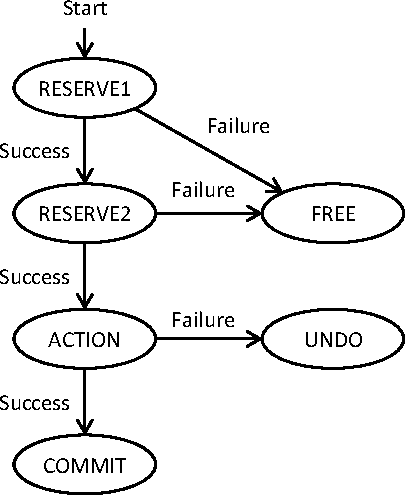
\includegraphics[scale=0.75]{bilder/zustandsdiagramm}
	\caption[Zustandsdiagramm der Modi in Net-SNMP]{Zustandsdiagramm der Modi in
	Net-SNMP. Quelle: \cite{NetSNMP11}}
	\label{fig:zustandsdiagramm}
\end{figure}

\section{Kompilation und Ausführung}
Das ganze Quellpaket von Net-SNMP wird benötigt. Beim Konfigurieren muss das
eigene, neue MIB-Module angeben werden. Nach dem Kompilieren gibt es die
Möglichkeit den Hintergrundprozess snmpd mit einfachen Methoden zu testen und
damit auch die Funktionalität des eigenen MIB-Moduls.

\chapter{Zusammenfassung und Ausblick}
Das Spektrum der Möglichkeiten sowie die Grenzen von Cacti sind anfangs
analysiert worden. Verschiedene methodisch-technische und Nutzen"-orientierte
Einsatzgebiete und der Gewinn der privaten Verwendung Cactis wurde dargelegt und
mit Anwendungsfällen untermauert, wie z.B.
Webserverabfragen, Monitoring für einen Voice-over-IP-Service, Visualierungen
von Sicherheitsbelangen und die Darstellung von Ressourcen. Es wurden die
üblichen Wege beschrieben Werte auszulesen. Dabei wurden Beispiele für
Bash-Scripte ausgewählt, die einen entsprechenden Nutzen bezogen zum jeweiligen
Dienst bieten. Die Funktionalität der Beispiele wurde anhand von Quelltexten und
Logdateien sukzessiv erklärt. Da es mit Cacti möglich ist auf SNMP-Dienste und
-Geräte zuzugreifen, wurde dargelegt, wie anstelle der vorgegebenen
Werteabfragen des NET-SNMP-Dienstes mit MIB-Modulen beliebige Abfragen
bewerkstelligbar sind.

Ursprünglich war die Cacti-Version 1.0 für das erste Quartal 2012 geplant.
Aktuell existiert die Version 0.8.8c. In Aussicht gestellt wird die
Implementierung der Web 2.0 Technologie AJAX, eine erweiterte Plugin-Architektur
und weitere integrierte Plugins, Verfügbarkeit von weiteren Sprachen,
erweitertes Templating und erweiterte Graphenvisualisierung. Die aktuelle
Version besitzt Fehler, wie man in der Übersicht der Fehlerkorrekturen erkennen
kann und ist für den professionellen Einsatz deshalb nur bedingt einsetzbar. Es
ist zu erwarten, dass in einer finalen Version Fehler beseitigt sein werden.

In danach erscheinenden Versionen ist ein Benutzer-Audit-Logging vorgesehen,
entferntes und dezentralisiertes Polling und ein Benutzergruppen- und
Rechtesystem innerhalb von Cacti.

Wünschenswert sind weitere Diagrammtypen, ein stärkerer mathematischer
realisierbarer Eingriff in die Wiedergabe des Graphen, eine Importfunktion von
bereits existierenden Werten und die automatische Positionierung von Text zu
Werten in Diagrammen. Letzteres ist nützlich, wenn bestimmte Ereignisse
zurückverfolgbar sein müssen. Anstelle eines Pollers ließe sich ein
Handshakeverfahren implementieren. Dies hat den Vorteil hat, dass nur
Datenverkehr aufkommt, sofern sich Werte ändern und sofern Tiefen und Spitzen in
einem Zeitfenster bedeutsam sind. Schließlich werden mit einem Poller lediglich
Werte im Minutenabstand abgefragt, wobei kürzere Zeitabstände als der
Pollerabstand nicht berücksichtigt werden. Hybridmodi eines Pollers oder eines
Handshake-Verfahrens gibt es in weiteren Monitoring-Lösungen.
\newpage
\begin{appendix}
\chapter{Grundaufbau eines MIB-Modules}
\label{appendix:GrundaufbauMIBModul}
Der Quelltext stammt aus \cite{NetSNMP11}

\begin{lstlisting}[numbers=left]
#include <net-snmp/net-snmp-config.h>
#include <net-snmp/net-snmp-includes.h>
#include <net-snmp/agent/net-snmp-agent-includes.h>

#include "delayed_instance.h"

static u_long delay_time = 1;

void init_delayed_instance(void)
{
  static oid  my_delayed_oid[] =
    { 1, 3, 6, 1, 4, 1, 8072, 2, 1, 2, 0 };
  netsnmp_handler_registration *my_test;

  my_test = netsnmp_create_handler_registration(
    "delayed_instance_example",
    delayed_instance_handler, my_delayed_oid,
    OID_LENGTH(my_delayed_oid), HANDLER_CAN_RWRITE);

  netsnmp_register_instance(my_test);
}

#define DELAYED_INSTANCE_SET_NAME "test_delayed"

int delayed_instance_handler(netsnmp_mib_handler *handler,
  netsnmp_handler_registration *reginfo,
  netsnmp_agent_request_info *reqinfo,
  netsnmp_request_info *requests)
{
  DEBUGMSGTL(("delayed_instance", "Got request, mode = %d:\n",
    reqinfo->mode));

  switch (reqinfo->mode) {
    default:
      requests->delegated = 1;
      
      snmp_alarm_register(delay_time, 0, return_delayed_response,   
        (void *) netsnmp_create_delegated_cache(handler, reginfo,
          reqinfo, requests, NULL));
        break;
  }
  return SNMP_ERR_NOERROR;
}

void return_delayed_response(unsigned int clientreg, void *clientarg)
{
  netsnmp_delegated_cache *cache = (netsnmp_delegated_cache *) clientarg;
  
  netsnmp_request_info *requests;
  netsnmp_agent_request_info *reqinfo;
  u_long *delay_time_cache = NULL;

  cache = netsnmp_handler_check_cache(cache);

  if (!cache) {
    snmp_log(LOG_ERR, "illegal call to return delayed response\n");
    return;
  }
  reqinfo = cache->reqinfo;
  requests = cache->requests;

  DEBUGMSGTL(("delayed_instance",
    "continuing delayed request, mode = %d\n", cache->reqinfo->mode));

  requests->delegated = 0;

  switch (cache->reqinfo->mode) {
    case MODE_GET:
    case MODE_GETNEXT:
      snmp_set_var_typed_value(cache->requests->requestvb,
        ASN_INTEGER, (u_char *) & delay_time, sizeof(delay_time));
        break;
    case MODE_SET_RESERVE1:
      if (requests->requestvb->type != ASN_INTEGER) {
        netsnmp_set_request_error(reqinfo, requests,
          SNMP_ERR_WRONGTYPE);
        netsnmp_free_delegated_cache(cache);
        return;
      }
      break;

    case MODE_SET_RESERVE2:
      memdup((u_char **) & delay_time_cache, (u_char *) &
        delay_time, sizeof(delay_time));

      if (delay_time_cache == NULL) {
        netsnmp_set_request_error(reqinfo, requests,
          SNMP_ERR_RESOURCEUNAVAILABLE);
        netsnmp_free_delegated_cache(cache);
        return;
      }
      netsnmp_request_add_list_data(requests,
        netsnmp_create_data_list (DELAYED_INSTANCE_SET_NAME,
          delay_time_cache, free));
      break;

    case MODE_SET_ACTION:
      delay_time = *(requests->requestvb->val.integer);
      DEBUGMSGTL(("testhandler", "updated delay_time -> %d\n",
        delay_time));
      break;

    case MODE_SET_UNDO:
      delay_time = *((u_long *) netsnmp_request_get_list_data(
        requests, DELAYED_INSTANCE_SET_NAME));
        break;

    case MODE_SET_COMMIT:
    case MODE_SET_FREE:
        break;
    }
    netsnmp_free_delegated_cache(cache);
}
\end{lstlisting}
\end{appendix}
\newpage

\bibliographystyle{abbrv}
\bibliography{literatur}
\addcontentsline{toc}{section}{Literatur}
%\addcontentsline{toc}{section}{\protect\numberline{A}{Literatur}}
\chapter*{}
\thispagestyle{empty}
\end{document}